%%%%%%%%%%%%%%%%%%%%%%%%%%%%%%%%%%%%%%%%%%%%%%%%%%%%%%%%%%%%%%%%%%%%%%%%%%
 %																		%
 %	Plantilla Latex para presentación del proyecto de curso				%
 %	Programación de Aplicaciones para Internet y la Nube					%
 %																		%
 %	Creada por: Duván Pardo, Wilson López								%
 %																		%
 %	Versión: 0.2															%
 %	Dapardoc@gmail.com ; Wilrilo@gmail.com								%
 %																		% 
 %	Se requieren los archivos  plantilla.bbl								% 
 %	El directorio Imagenes que contiene: CECAD,DC, Elementos y RITA		%  
 %																		%
%%%%%%%%%%%%%%%%%%%%%%%%%%%%%%%%%%%%%%%%%%%%%%%%%%%%%%%%%%%%%%%%%%%%%%%%%%

\documentclass[10pt]{article}   			% Describe el tipo de documento, y el tamaño de la letra del texto

\usepackage[utf8]{inputenc}				% Define codificación para que permita caracteres latinos (acentos)
\usepackage[spanish,activeacute]{babel} 	% Paquete para poder escribir con tildes y otros caracteres especiales

\usepackage{vmargin}						% Código para margenes y formato de página
\setpapersize{A4}
\setmargins	{2.2cm}     					% margen izquierdo
			{1 cm}                 		% margen superior
			{16.5cm}               		% anchura del texto
			{23.42cm}             		% altura del texto
			{20pt}                		% altura de los encabezados
			{1.2cm}               		% espacio entre el texto y los encabezados
			{0pt}                		% altura del pie de página
			{2cm}                 		% espacio entre el texto y el pie de página

\usepackage{amsmath}						% paquete para expresiones matemáticas
\usepackage{amsfonts}					% paquete para escritura de ecuaciones 
\usepackage{amssymb}						% paquete para caracteres especiales para ecuaciones 

\usepackage{fancyhdr}					% Temas para encabezado y pie de pagina
\usepackage{fancyvrb}
\pagestyle{fancy} 

\pagenumbering{arabic} 					% Numeración de paginas {arabic roman}
\usepackage{hyperref}					% Para hipervinculos
\usepackage{graphicx}					% Para incluir imágenes
\usepackage{caption}						% Descripciones de las figuras
\usepackage{subcaption}					% Descripción varias imagenes en usa sola figura
\graphicspath{ {Imagenes/} }				% Directorio de imágenes esta capeta va donde esta el archivo tex


\usepackage{color, colortbl}				% Colores para tablas
\usepackage{listings}					% Para el código Fuente
\usepackage{xcolor}						% para color en codigos o listrings
\definecolor{limegreen}{RGB}{50,100,50}	% Definición de colores ejemplo verde en RGB
\definecolor{Red}{RGB}{220,120,120}		% se definen colores para la tabla en el cronograma pueden ser RGB 0-255 o rgb 0-1 cada componente
\definecolor{LightCyan}{rgb}{0.88,1,1}
\definecolor{azul}{RGB}{120,120,210}
\lstdefinestyle{base}{
	language=C,
	emptylines=1,
	breaklines=true,
	showspaces=fasle,
	showstringspaces=false,
	extendedchars=true,
	basicstyle=\ttfamily\color{black},
	moredelim=**[is][\color{limegreen}]{'}{'}, 	% Para este caso especial el caracter ' y & encierran
	moredelim=**[is][\color{blue}]{&}{&},		% un fragmento de código que quiere ser coloreado
}

\lstset{numbers=left, numberstyle=\tiny, stepnumber=2, numbersep=5pt}

%Aquí inicia el documento.
\begin{document}
	% Se define el Encabezado
	%clhead[]{Proyecto}
	\lhead[]{Programación de Aplicaciones para Internet y la Nube}
	\rhead[]{\textbf{2016-I}}
	\renewcommand{\headrulewidth}{0.5pt}

	\thispagestyle{empty}						% La primera página no lleva estilo (sin encabezado)
	\begin{center}
		\large {Programación de Aplicaciones para Internet y la Nube
			\hspace{5 cm}\textbf{2016-I}}
		\bigskip  
		\textbf{
			\LARGE{\\TALLERES}}\\								% Nombre del proyecto
	\end{center}	
	\begin{flushright}	
		\bigskip	
		Nombre del Estudiante: \textbf{Andres Julian Moreno, Yeny Katherine Muñoz}			% Nombre del estudiante
	\end{flushright} 
	
\section{Taller 1 - IaaS - Orquestación en Opestack - Parte I}

El objetivo del primer taller, fue realizar despliegues de infraestructura sencillos utilizando el lenguaje de orquestación de OpenStack. Para llevar a cabo está actividad se realizó el siguiente procedimiento:

\begin{itemize}		
\item Crear un archivo denominado “router.yaml” con el siguiente contenido. 
\begin{small}
\begin{lstlisting}[frame=single,style=base]	
&heat_template_version: 2015-04-30&

&description:& Desarrollo del taller &1& app en la nube

&parameters:&

  &public_network:&
    &type:& string
    &label:& Public network with name or ID
    &description:& Public network with floating IP addresses
    &default:& ext-net-doctorado

&resources:&

  &router:&
    &type:& OS::Neutron::Router
    &properties:&
      &external_gateway_info:&
        &network:& { &get_param:& public_network }
\end{lstlisting}
\end{small}

\item Verificar la correcta creación del router.
\begin{figure}[ht] 
	\centering
		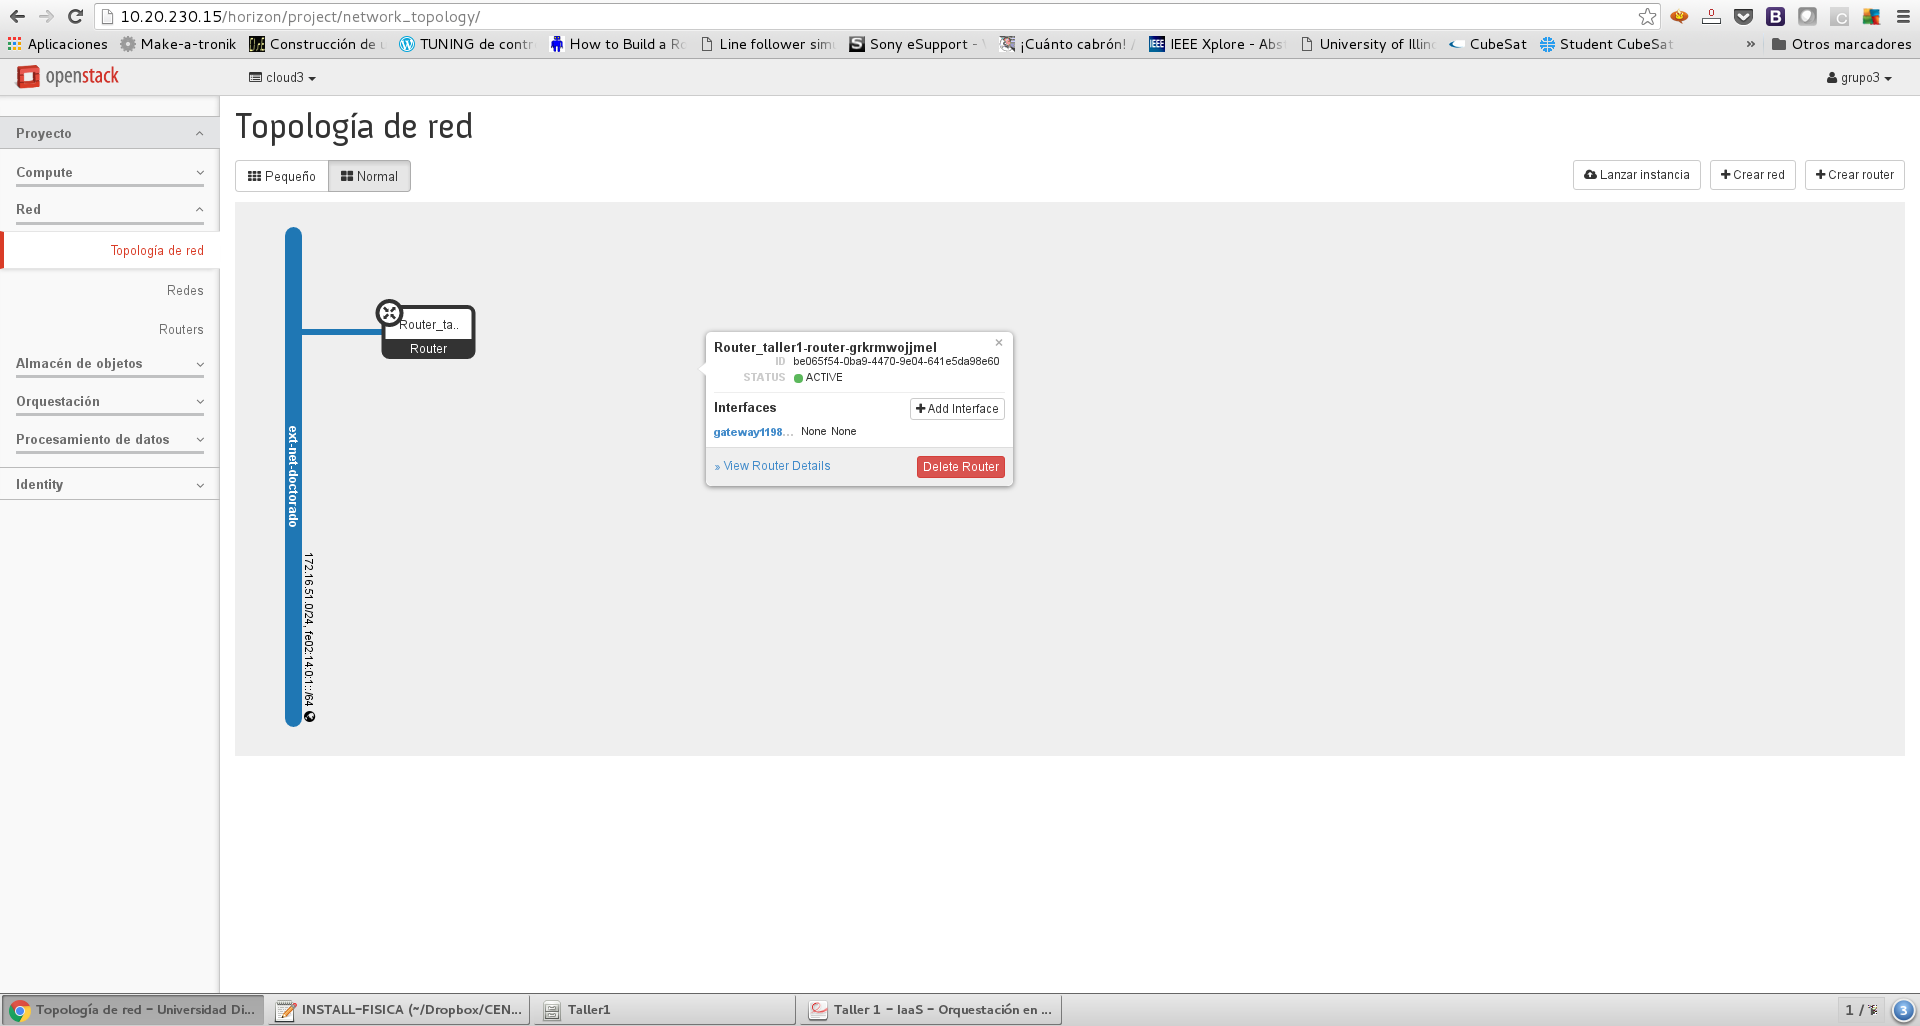
\includegraphics[scale=0.27]{router}   
	\caption{Creación del router en horizon} \label{fig:Router}
\end{figure}

\item Crear un archivo denominado “network.yaml” con el siguiente contenido y ejecutar la plantilla.
\begin{small}
\begin{lstlisting}[frame=single,style=base]	
&heat_template_version: 2015-04-30&

&description:& Desarrollo del taller &1& app en la nube

&parameters:&

  &private_network_cidr:&
    &type:& string
    &label:& Private network CIDR
    &description:& Private Network CIDR
    &default: 192.168.200.0/24&

&resources:&

   &private_network:&
     &type:& OS::Neutron::Net

   &private_subnet:&
     &type:& OS::Neutron::Subnet
     &properties:&
       &network_id:& { &get_resource:& private_network }
       &cidr:& {&get_param:& private_network_cidr}
       &dns_nameservers:& 
        - &8.8.8.8&
\end{lstlisting}
\end{small}

\item Verificar la correcta creación de la red.
\begin{figure}[ht] 
	\centering
		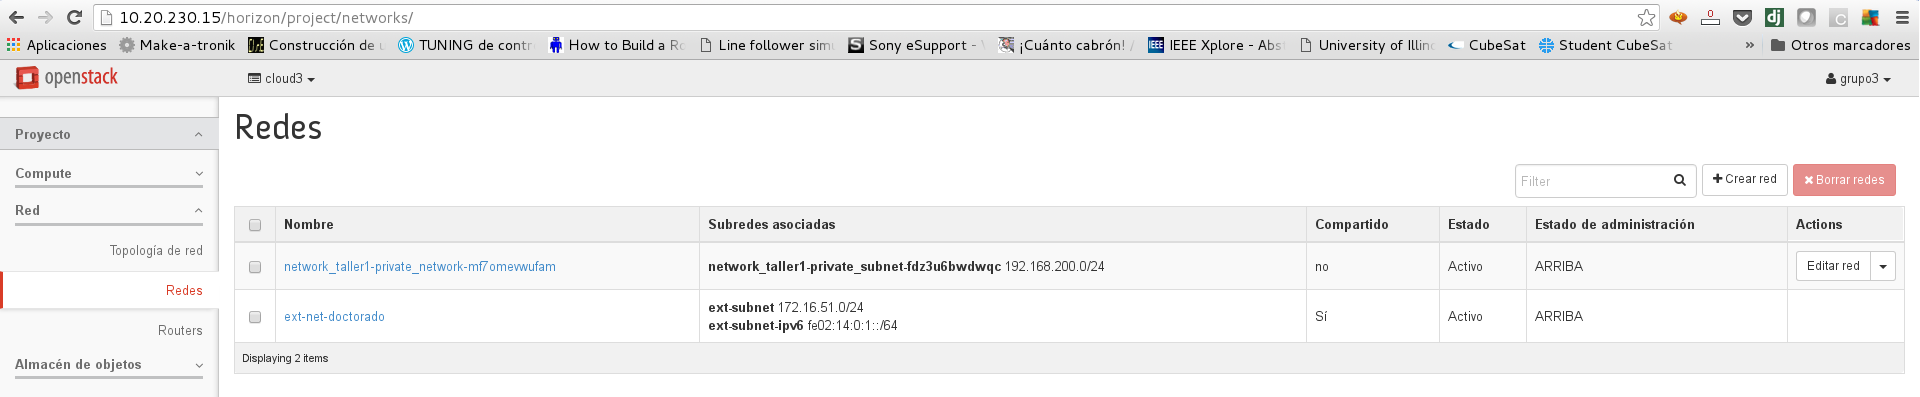
\includegraphics[scale=0.27]{network} 
 		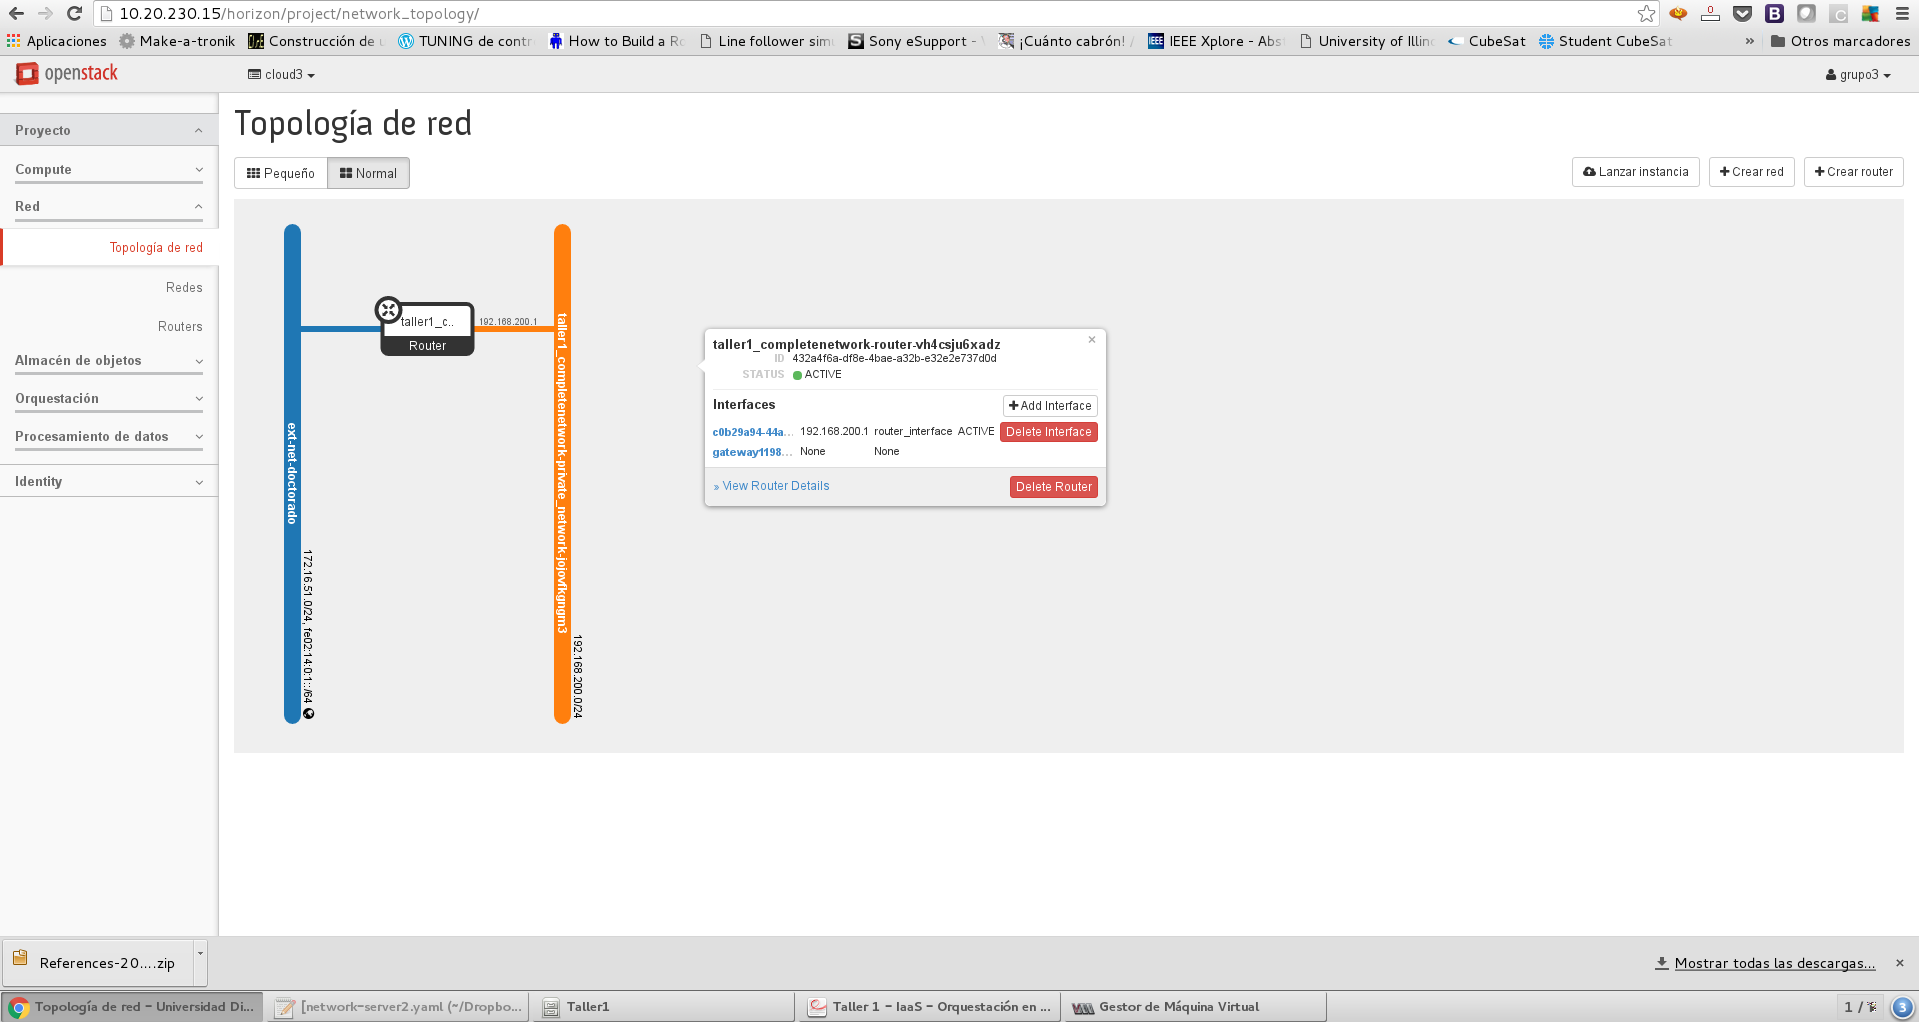
\includegraphics[scale=0.27]{complete-network} 
	\caption{Creación de la red en horizon} \label{fig:Network}
\end{figure}

\item Eliminar las pilas previamente creadas.
\item Crear un archivo denominar “complete-network.yaml” con el siguiente contenido y ejecutar la plantilla. En este paso, se va a crear un router, una red privada, y se le va a asignar un puerto al router dentro de esa red.
\begin{small}
\begin{lstlisting}[frame=single,style=base]	
&heat_template_version: 2015-04-30&

&description:& Desarrollo del taller &1& app en la nube

&parameters:&

  &public_network:&
    &type:& string
    &label:& Public network with name or ID
    &description:& Public network with floating IP addresses
    &default:& ext-net-doctorado

  &private_network_cidr:&
    &type:& string
    &label:& Private network CIDR
    &description:& Private Network CIDR
    &default: 192.168.200.0/24&

&resources:&

  &router:&
    &type:& OS::Neutron::Router
    &properties:&
      &external_gateway_info:&
        &network:& { &get_param:& public_network }

  &private_network:&
     &type:& OS::Neutron::Net

  &private_subnet:&
     &type:& OS::Neutron::Subnet
     &properties:&
       &network_id:& { &get_resource:& private_network }
       &cidr:& {&get_param:& private_network_cidr}
       &dns_nameservers: 
        - 8.8.8.8&

  &router-interface:&
     &type:& OS::Neutron::RouterInterface
     &properties:&
       &router_id:& { &get_resource:& router }
       &subnet:& { &get_resource:& private_subnet }
\end{lstlisting}
\end{small}

Una vez la creada infraestructura de red, el siguiente paso es crear servidores. Inicialmente, se desplegará únicamente el servidor con su respectivo grupo de seguridad. Posteriormente se le configurará en la plantilla el software a instalar y se le asignará un IP flotante.

\item Eliminar las pilas previamente creadas.
\item Crear un archivo denominar “network-server.yaml” con el siguiente contenido y ejecutar la plantilla. En este paso, se va a crear un router, una red privada, se le va a asignar un puerto al router dentro de esa red, y se va a lanzar una instancia con un grupo de seguridad y una llave.
\begin{small}
\begin{lstlisting}[frame=single,style=base]	
&heat_template_version: 2015-04-30&

&description:& Desarrollo del taller &1& app en la nube

&parameters:&

  &public_network:&
    &type:& string
    &label:& Public network with name or ID
    &description:& Public network with floating IP addresses
    &default:& ext-net-doctorado

  &private_network_cidr:&
    &type:& string
    &label:& Private network CIDR
    &description:& Private Network CIDR
    &default: 192.168.200.0/24&

  &image:&
    &type:& string
    &label:& Image name or ID
    &description:& Image to be used for compute instance
    &default:& ubuntu-server&-14.04&-CECAD-r20141201

  &flavor:&
    &type:& string
    &label:& Flavor
    &description:& Type of instance to be used
    &default:& m1.small

&resources:&

  &router:&
    &type:& OS::Neutron::Router
    &properties:&
      &external_gateway_info:&
        &network:& { &get_param:& public_network }

  &private_network:&
     &type:& OS::Neutron::Net

  &private_subnet:&
     &type:& OS::Neutron::Subnet
     &properties:&
       &network_id:& { &get_resource:& private_network }
       &cidr:& {&get_param:& private_network_cidr}
       &dns_nameservers:& 
        - &8.8.8.8&

  &router-interface:&
     &type:& OS::Neutron::RouterInterface
     &properties:&
       &router_id:& { &get_resource:& router }
       &subnet:& { &get_resource:& private_subnet } 

  &web_server_security_group:&
     &type:& OS::Neutron::SecurityGroup
     &properties:&
       &name:& web_server_security-group
       &rules:&
         - &protocol:& tcp
           &port_range_min: 80&
           &port_range_max: 80&
         - &protocol:& tcp
           &port_range_min: 443&
           &port_range_max: 443&
         - &protocol:& icmp
         - &protocol:& tcp
           &port_range_min: 22&
           &port_range_max: 22&

  &my_keypair:&
    &type:& OS::Nova::Server
    &properties:&
      &name:& cloudapps
      &save_private_key: True&

  &my_instance:&
    &type:& OS::Nova::Server
    &properties:&
      &image:& { &get_param:& image }
      &flavor:& { &get_param:& flavor }
      &key_name:& { &get_resource:& my_keypair }
      &networks:&
        - &network:& { &get_resource:& private_network }
      &security_groups:&
        - { &get_resource:& web_server_security_group }
      &user_data:& | 
        '#!/bin/sh
	sudo apt-get -y update && sudo apt-get -y install apache2 && sudo service apache2 restart'
      &user_data_format:& RAW

  &outputs:&
      &my_instance_name:&
        &description:& Name of the instance
        &value:& { &get_attr:& [my_instance, name] }
      &my_instance_ip:&
        &description:& IP of the instance
        &value:& { &get_attr:& [my_instance, first_address] }
\end{lstlisting}
\end{small}

\item Finalmente, se le va a asignar una IP flotante a la instancia. Modificar el archivo “network-server.yaml” en la sección “resources” para que luzca de la siguiente forma:
\begin{small}
\begin{lstlisting}[frame=single,style=base]	
&heat_template_version: 2015-04-30&

&description:& Desarrollo del taller &1& app en la nube

&parameters:&

  &public_network:&
    &type:& string
    &label:& Public network with name or ID
    &description:& Public network with floating IP addresses
    &default:& ext-net-doctorado

  &private_network_cidr:&
    &type:& string
    &label:& Private network CIDR
    &description:& Private Network CIDR
    &default: 192.168.200.0/24&

  &image:&
    &type:& string
    &label:& Image name or ID
    &description:& Image to be used for compute instance
    &default:& ubuntu-server&-14.04&-CECAD-r20141201

  &flavor:&
    &type:& string
    &label:& Flavor
    &description:& Type of instance to be used
    &default:& m1.small

&resources:&

  &router:&
    &type:& OS::Neutron::Router
    &properties:&
      &external_gateway_info:&
        &network:& { &get_param:& public_network }

  &private_network:&
     &type:& OS::Neutron::Net

  &private_subnet:&
     &type:& OS::Neutron::Subnet
     &properties:&
       &network_id:& { &get_resource:& private_network }
       &cidr:& {&get_param:& private_network_cidr}
       &dns_nameservers:& 
        - &8.8.8.8&

  &router-interface:&
     &type:& OS::Neutron::RouterInterface
     &properties:&
       &router_id:& { &get_resource:& router }
       &subnet:& { &get_resource:& private_subnet } 

  &web_server_security_group:&
     &type:& OS::Neutron::SecurityGroup
     &properties:&
       &name:& web_server_security-group
       &rules:&
         - &protocol:& tcp
           &port_range_min: 80&
           &port_range_max: 80&
         - &protocol:& tcp
           &port_range_min: 443&
           &port_range_max: 443&
         - &protocol:& icmp
         - &protocol:& tcp
           &port_range_min: 22&
           &port_range_max: 22&

  &my_keypair:&
    &type:& OS::Nova::Server
    &properties:&
      &name:& cloudapps
      &save_private_key: True&

  &floating_ip:&
    &type:& OS::Neutron::FloatingIP
    &properties:&
      &floating_network:& { &get_param:& public_network } 

  &server_port:&
    &type:& OS::Neutron::Port
    &properties:&
      &network:& { &get_resource:& private_network }
      &security_groups:&
        - { &get_resources:& web_server_security_group } 

  &my_instance:&
    &type:& OS::Nova::Server
    &properties:&
      &image:& { &get_param:& image }
      &flavor:& { &get_param:& flavor }
      &key_name:& { &get_resource:& my_keypair }
      &networks:&
        - &network:& { &get_resource:& private_network }
      &security_groups:&
        - { &get_resource:& web_server_security_group }
      &user_data:& | 
        '#!/bin/sh
	sudo apt-get -y update && sudo apt-get -y install apache2 && sudo service apache2 restart'
      &user_data_format:& RAW

  &floating_ip_assoc:&
    &type:& OS::Neutron::FloatingIPAssociation
    &properties:&
      &floatingip_id:& { &get_resourse:& floating_ip }
      &port_id:& { &get_resource:& server_port }

\end{lstlisting}
\end{small}

\item Esperar un breve tiempo y acceder a la página pre-establecida de Apache direccionando cualquier explorador a la dirección:  \href{http://192.168.200.0}{http://"ip-flotante-instancia".}

\begin{figure}[ht]
\centering
\begin{subfigure}[b]{0.4\textwidth}  		% el nunero se utiliza para cambiar la escala de la imagne
	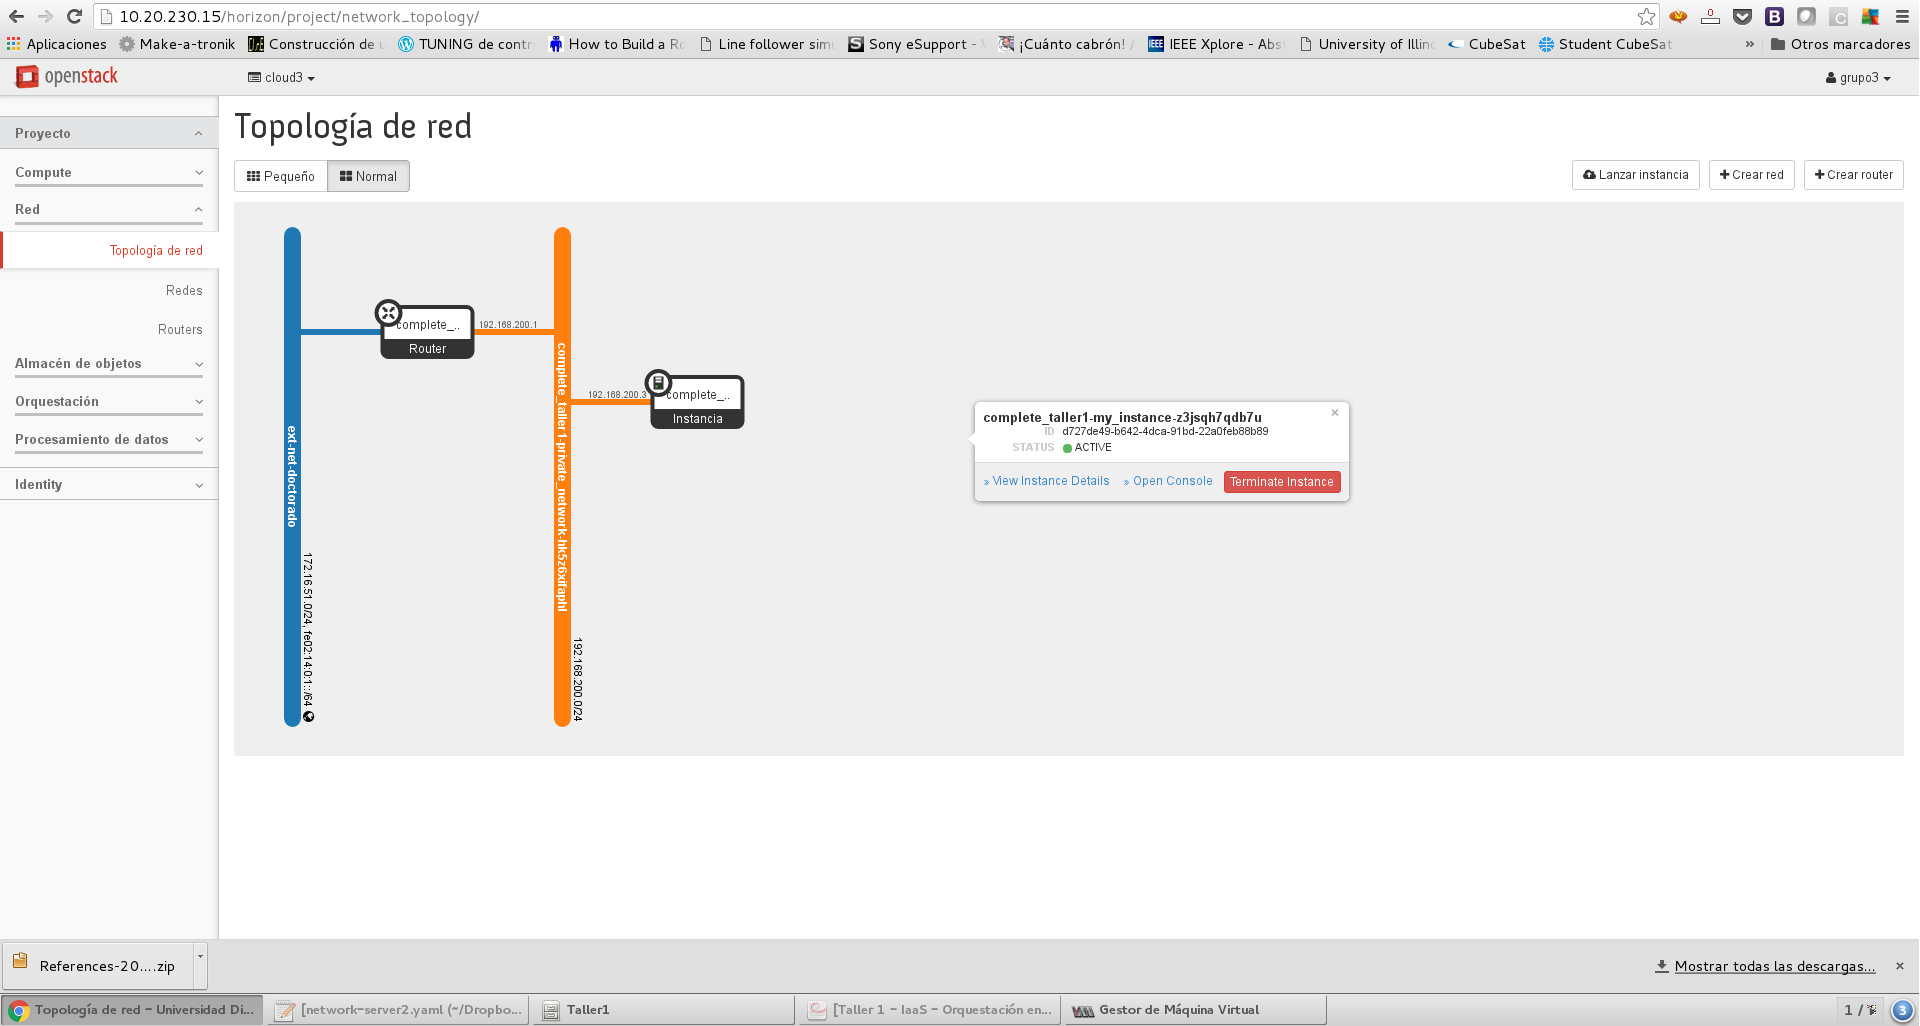
\includegraphics[width=\textwidth]{redfinal}
	\caption{Red final}
	\label{fig:redfinal}
\end{subfigure}
\begin{subfigure}[b]{0.4\textwidth}		 	% el nunero se utiliza para cambiar la escala de la imagne
	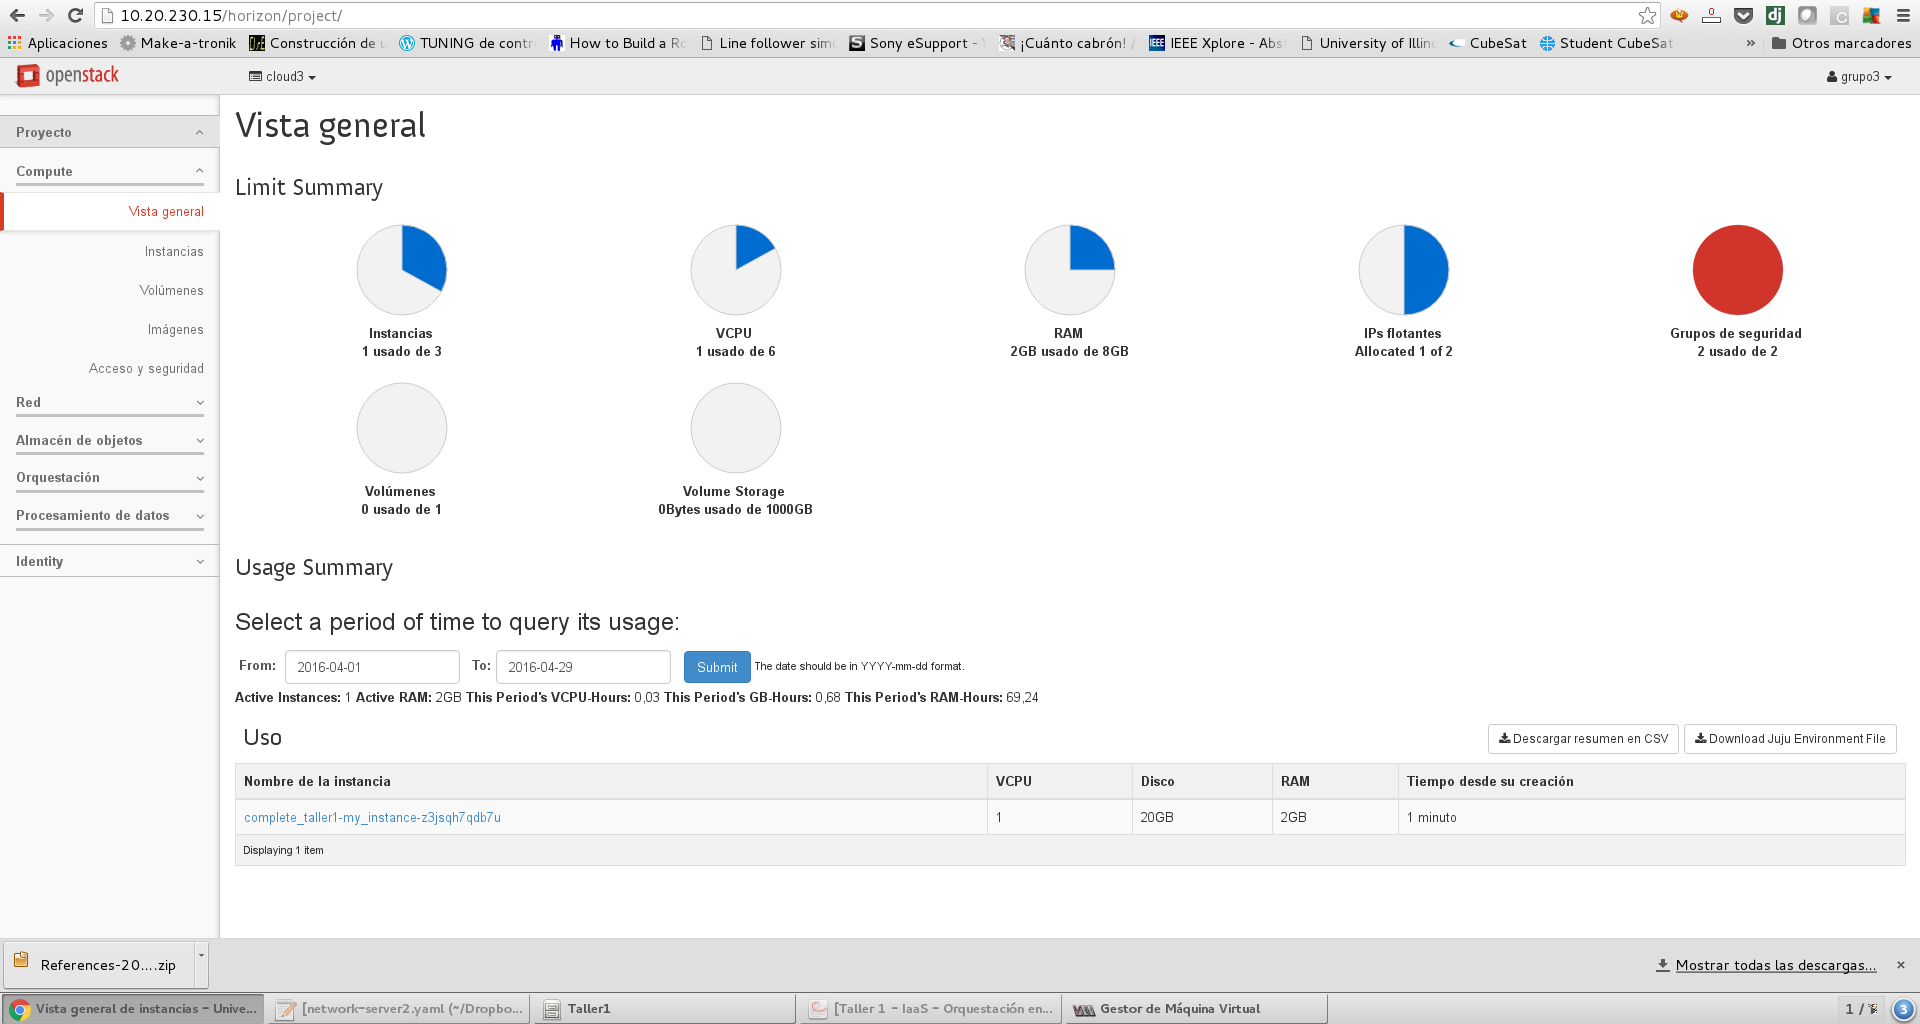
\includegraphics[width=\textwidth]{recursosfinal}
	\caption{Uso de recursos final}
	\label{fig:recursosfinal}
\end{subfigure}
\begin{subfigure}[b]{0.8\textwidth}		 	% el nunero se utiliza para cambiar la escala de la imagne
	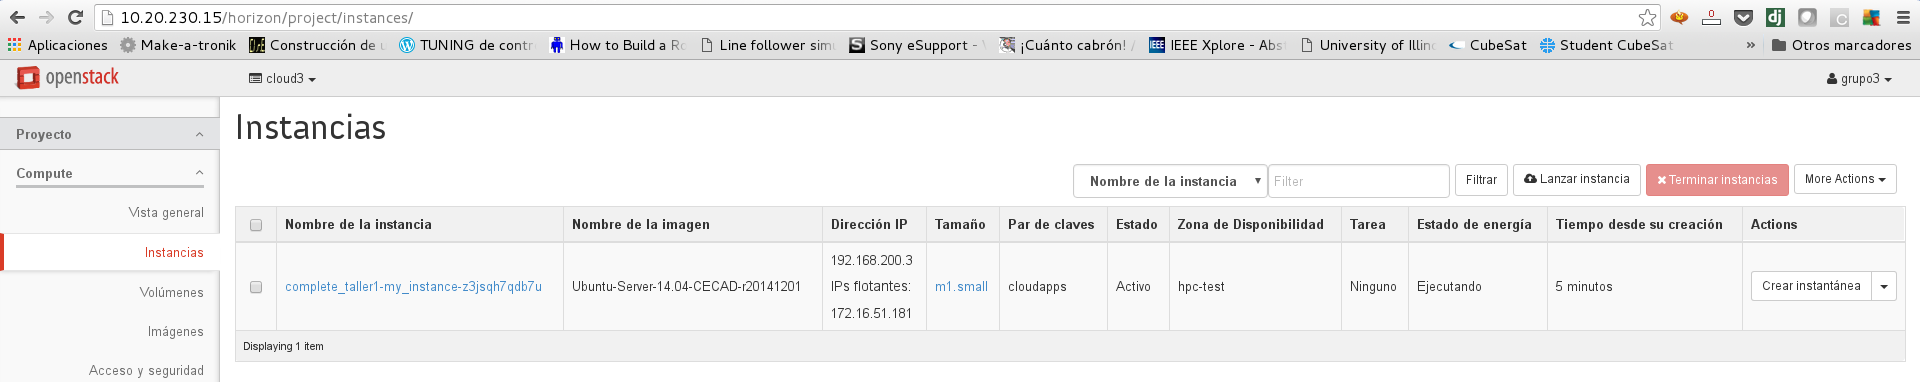
\includegraphics[width=\textwidth]{instanciafinal}
	\caption{Instancia final}
	\label{fig:instanciafinal}
\end{subfigure}
\begin{subfigure}[b]{0.8\textwidth}		 	% el nunero se utiliza para cambiar la escala de la imagne
	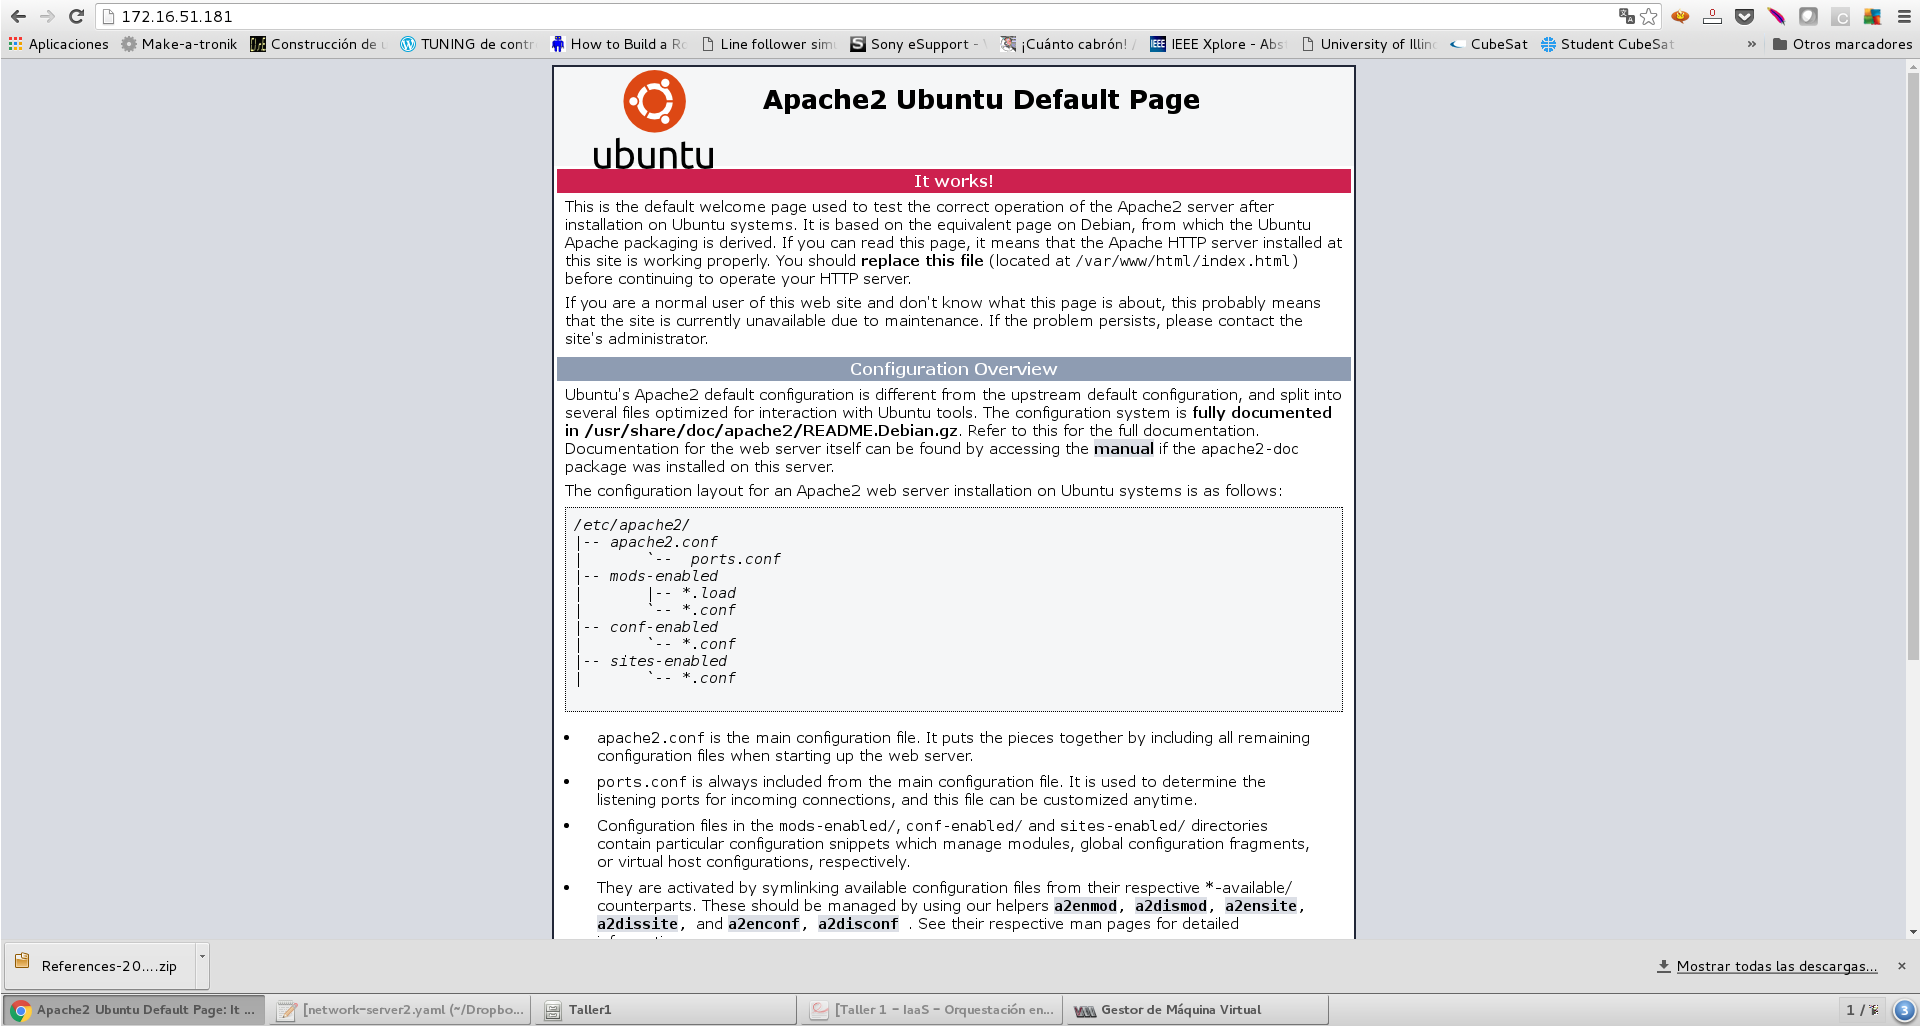
\includegraphics[width=\textwidth]{apache}
	\caption{Página pre-establecida de apache}
	\label{fig:apache}
\end{subfigure}

\caption{Acceso página pre-establecida de Apache}\label{fig:Apache}

\end{figure}

\end{itemize}

\newpage % Se utiliza para escribir en una nueva pagina (estilo)

\section{Taller 2 - IaaS - Orquestación en Opestack - Parte II}

El objetivo del segundo taller, implica realizar despliegues de infraestructura utilizando el lenguaje de orquestación de OpenStack. En particular, realizar un despliegue multi-instancia cuyos servicios deben colaborar.
		
\begin{itemize}
	\item Crear un directorio “wordpress-openstack”, y dentro de ese directorio, un sub-directorio “lib”.
	\item Descargar los archivos mysql.yaml, wordpress.yaml, private-network.yaml, floating-ip.yaml en el directorio “lib”.
	\begin{figure}[ht] 
		\centering
			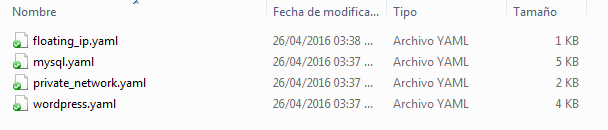
\includegraphics[scale=0.9]{lib}   
		\caption{Archivos descargados sobre carpeta lib} \label{fig:Librerias}
	\end{figure}

	\item Editar el archivo lib/private-network.yaml de forma que tenga el siguiente contenido:
	\begin{small}
	\begin{lstlisting}[frame=single,style=base]	
&heat_template_version: 2013-05-23&

&description:& Template that creates a private network.

&parameters:&
  &public_network:&
    &type:& string
    &label:& Public network name or ID
    &description:& Public network with floating IP addresses.
    &default:& public
  &cidr:&
    &type:& string
    &label:& CIDR
    &description:& The CIDR of the private network.
    &default:& '10.10.10.0/24'
  &dns:&
    &type:& comma_delimited_list
    &label:& DNS nameservers
    &description:& Comma separated list of DNS nameservers for the private network.
    &default:& '8.8.8.8'

&resources:&
  &private_network:&
    &type:& OS::Neutron::Net

  &private_subnet:&
    &type:& OS::Neutron::Subnet
    &properties:&
      &network_id:& { &get_resource:& private_network }
      &cidr: 10.10.10.0/24&
      &dns_nameservers:& { &get_param:& dns }

  &router:&
    &type:& OS::Neutron::Router
    &properties:&
      &external_gateway_info:&
        &network:& { &get_param:& public_network }

  &router-interface:&
    &type:& OS::Neutron::RouterInterface
    &properties:&
      &router_id:& { &get_resource:& router }
      &subnet:& { &get_resource:& private_subnet }

&outputs:&
  &name:&
    &description:& The private network.
    &value:& { &get_attr:& [private_network, name] }
	\end{lstlisting}
	\end{small}

Algo interesante del enfoque planteado en este laboratorio es utilizar las plantillas previamente definidas como cajas negras, funcionalidades ya probadas de quienes únicamente interesa sus entradas y sus salidas. Este enfoque se denomina “plantillas anidadas” y provee una manera más extensible de depurar los diferentes despliegues orquestados.
		
	\item Descargar el archivo heat-3d.yaml y ubicarlo en el directorio “wordpress-openstack”.
	\item Realizar las modificaciones al archivo, de forma que luzca como sigue a continuación:
	\begin{small}
	\begin{lstlisting}[frame=single,style=base]	
&heat_template_version: 2013-05-23&

&description:& Template that installs a wordpress server and supporting MySQL database running on separate servers.

&parameters:&
  &image:&
    &type:& string
    &label:& Image name or ID
    &description:& Image to be used for server. Please use an Ubuntu based image.
    &default:& ubuntu-Server&-14.04&-CECAD-r20141201
  &flavor:&
    &type:& string
    &label:& Flavor
    &description:& Type of instance (flavor) to be used on the compute instance.
    &default:& m1.small
  &key:&
    &type:& string
    &label:& Key name
    &description:& Name of key-pair to be installed on the compute instance.
    &default:& my_key
  &public_network:&
    &type:& string
    &label:& Public network name or ID
    &description:& Public network to attach server to.
    &default:& public
 
&resources:&
  &network:&
    &type:& Lib::MSG::PrivateNetwork
    &properties:&
      &public_network:& { &get_param:& public_network }

  &mysql:&
    &type:& Lib::MSG::MySQL
    &properties:&
      &image:& { &get_param:& image }
      &flavor:& { &get_param:& flavor }
      &key:& { &get_param:& key }
      &private_network:& { &get_attr:& [network, name] }
      &database_name:& wordpress
      &database_user:& wordpress_user
 
  &wordpress:&
    &type:& Lib::MSG::Wordpress
    &properties:&
      &image:& { &get_param:& image }
      &flavor:& { &get_param:& flavor }
      &key:& { &get_param:& key }
      &private_network:& { &get_attr:& [network, name] }
      &mysql_server:& { &get_attr:& [mysql, ip] }
      &database_name:& wordpress
      &database_user:& wordpress_user
      &database_password:& { &get_attr:& [mysql, database_password] }

  &floating_ip:&
    &type:& Lib::MSG::FloatingIP
    &properties:&
      &port:& { &get_attr:& [wordpress, port] }
      &public_network:& { &get_param:& public_network }

&outputs:&
  &ip:&
    &description:& The public IP address to access Wordpress.
    &value:& { &get_attr:& [floating_ip, ip] }
	\end{lstlisting}
	\end{small}

	\item Descargar el archivo env.yaml en el directorio “wordpress-openstack” y editarlo teniendo en cuenta la direcciones absolutas de los archivos *.yaml.
		\begin{figure}[ht] 
		\centering
			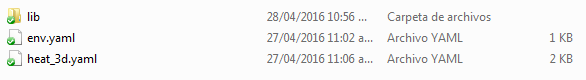
\includegraphics[scale=0.9]{wordpress}   
		\caption{Archivos descargados sobre la carpeta Wordpress Openstack} \label{fig:Wordpress}
	\end{figure}

	\item Lanzar la pila y acceder a la consola de Wordpress en la dirección de IP flotante asignada por la orquestación.
			
\end{itemize}
			
\newpage % Se utiliza para escribir en una nueva pagina (estilo)

\section{Taller 3 - IaaS - Fundamentos de Vagrant - Parte I}

El objetivo del tercer taller, desarrolla el despliegue de entornos de desarrollo sencillos mediante la tecnología Vagrant utilizando como proveedor de infraestructura la tecnología VirtualBox.

\begin{itemize}		

\item Abrir una consola de comandos. 
\item Validar la correcta instalación del software Vagrant ejecutando el comando "vagrant –h"
\begin{figure}[ht] 
	\centering
		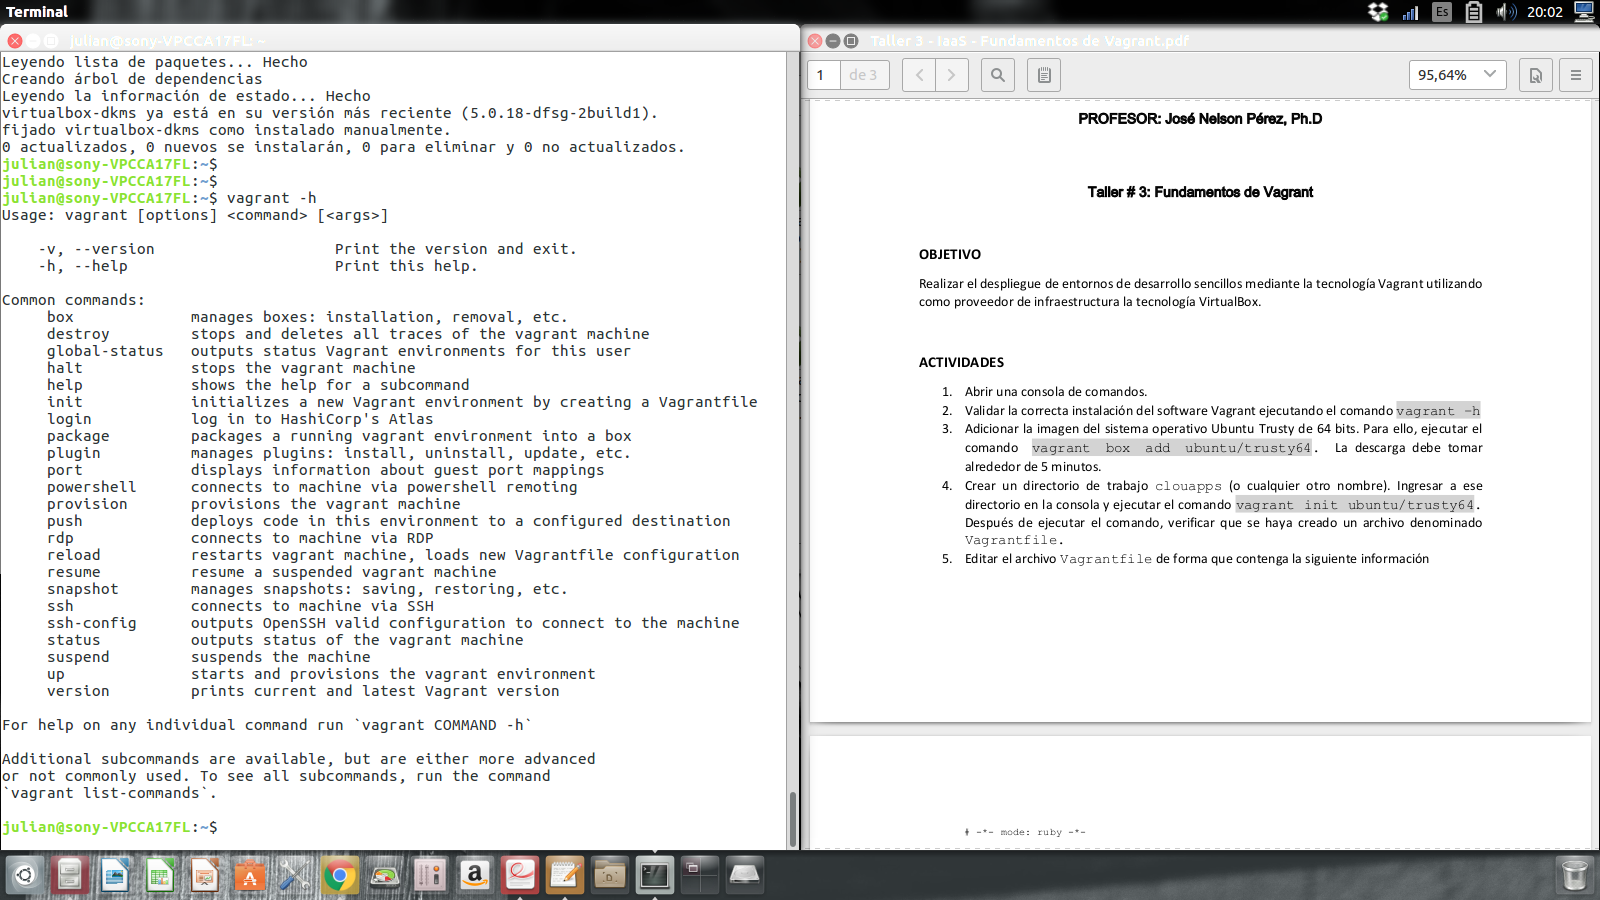
\includegraphics[scale=0.25]{vagrantverification}   
	\caption{Validación de la correcta instalación del software Vagrant} \label{fig:vagrantverification}
\end{figure}

\item Adicionar la imagen del sistema operativo Ubuntu Trusty de 64 bits. Para ello, ejecutar el comando "vagrant box add ubuntu/trusty64". La descarga debe tomar alrededor de 5 minutos.
\begin{figure}[ht] 
	\centering
		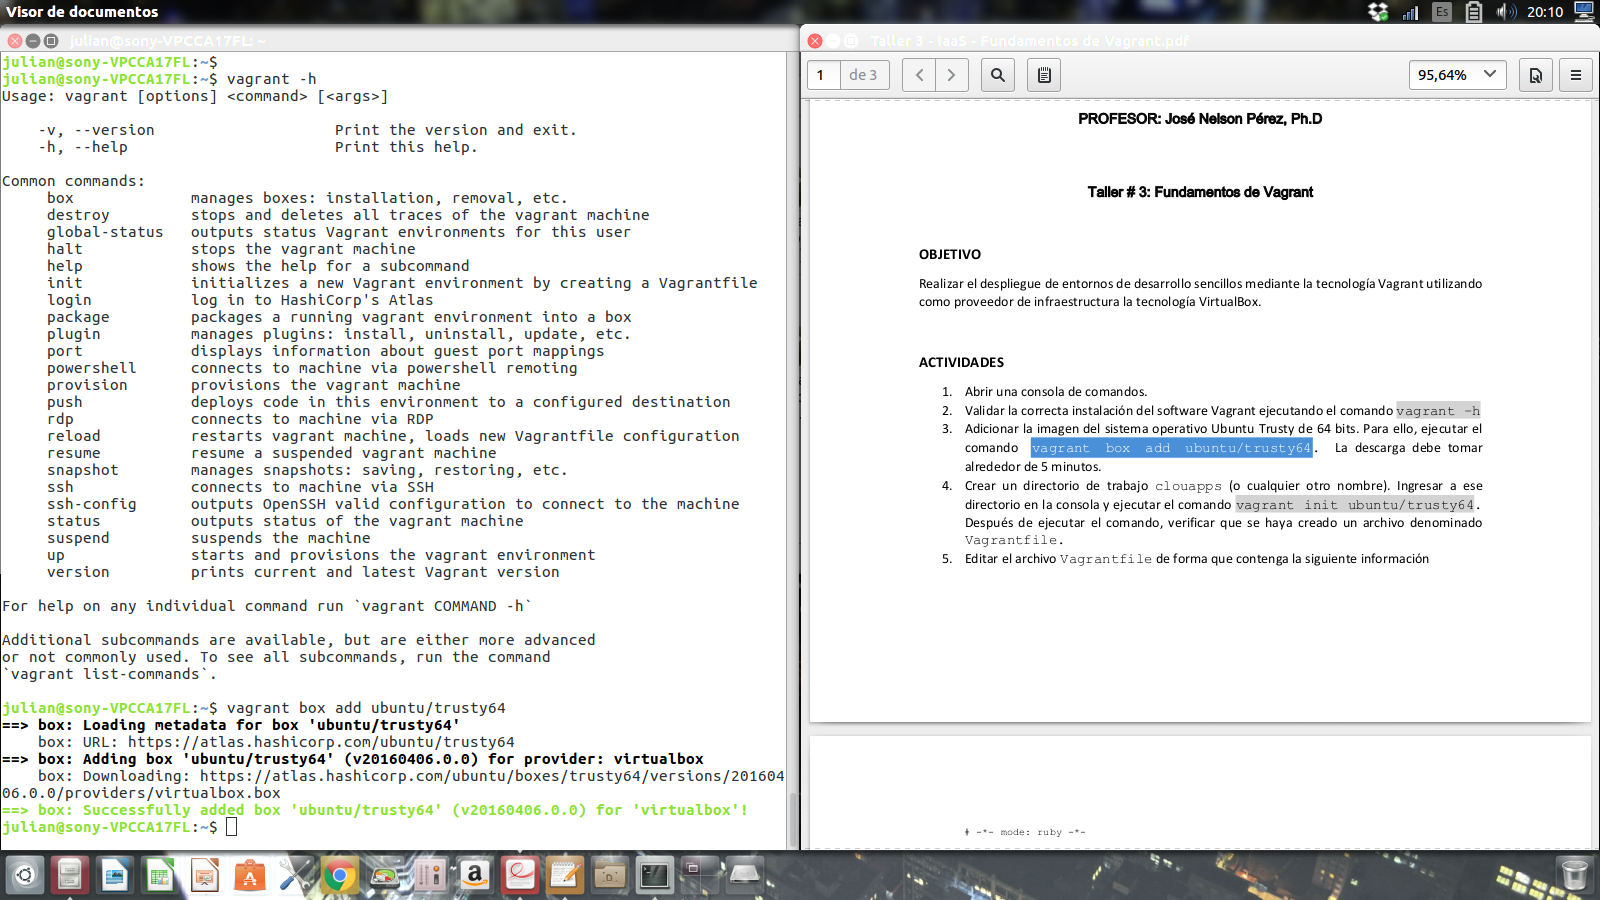
\includegraphics[scale=0.25]{bajadoubuntu}   
	\caption{Imagen del sistema operativo Ubuntu} \label{fig:bajadoubuntu}
\end{figure}

\item Crear un directorio de trabajo clouapps (o cualquier otro nombre). Ingresar a ese directorio en la consola y ejecutar el comando "vagrant init ubuntu/trusty64". Después de ejecutar el comando, verificar que se haya creado un archivo denominado "Vagrantfile".
\begin{figure}[ht] 
	\centering
		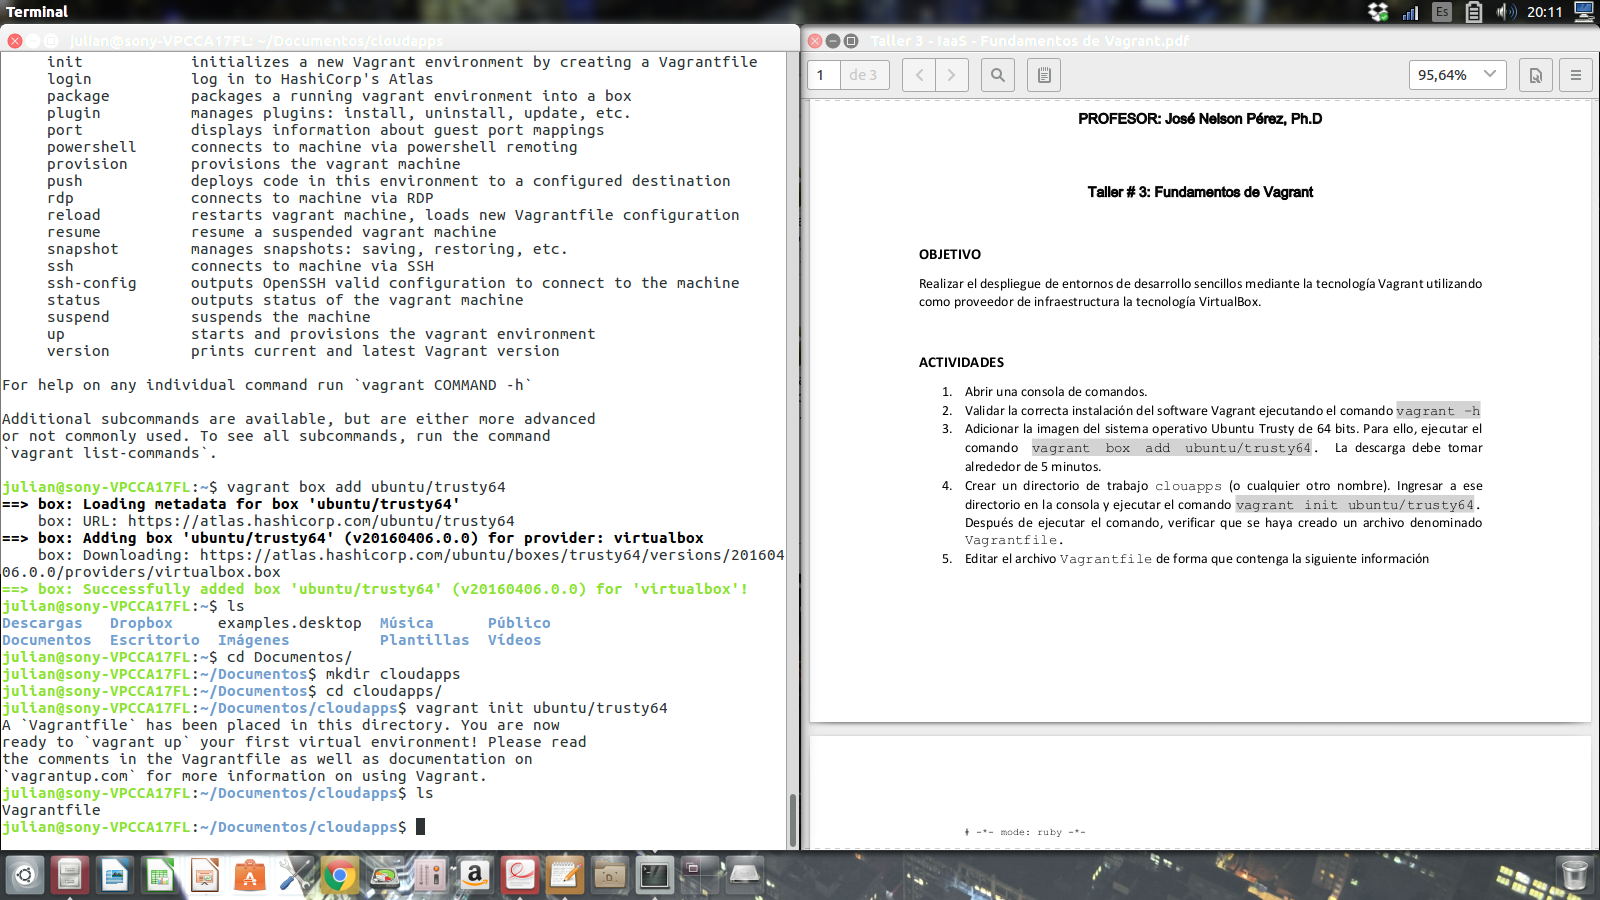
\includegraphics[scale=0.25]{vagrantfile}   
	\caption{ Creación del archivo denominado "Vagrantfile"} \label{fig:vagrantfile}
\end{figure}

\item Editar el archivo "Vagrantfile" de forma que contenga la siguiente información
	\begin{small}
	\begin{lstlisting}[frame=single,style=base]	
# -*- mode: ruby -*-
# vi: set ft=ruby :
# All Vagrant configuration is done below. The "2" in Vagrant.configure
# configures the configuration version (we support older styles for
# backwards compatibility). Please don't change it unless you know what
# you're doing.
Vagrant.configure(2) do |config|
config.vm.box = "ubuntu/trusty64"
config.vm.network :forwarded_port, guest: 4000, host: 8100, host_ip: "127.0.0.1"
config.vm.provision "shell", path: "script.sh"
end
	\end{lstlisting}
	\end{small}

\item Crear un archivo “script.sh” en el mismo directorio del archivo "Vagrantfile".
\item Escribir el siguiente contenido en el archivo “script.sh”.
	
\begin{small}
	\begin{lstlisting}[frame=single,style=base]	
#!/usr/bin/env bash
echo "Installing: nodejs, lynx, ruby and jekyll..."
apt-add-repository ppa:brightbox/ruby-ng >>/tmp/provision-script.log 2>&1&
apt-get -y update >>/tmp/provision-script.log 2>&1&
apt-get install -y nodejs >>/tmp/provision-script.log 2>&1&
apt-get install -y lynx-cur >>/tmp/provision-script.log 2>&1&
apt-get install -y ruby2.2 >>/tmp/provision-script.log 2>&1&
apt-get install -y ruby2.2-dev >>/tmp/provision-script.log 2>&1&
gem install jekyll >>/tmp/provision-script.log 2>&1&
cd /vagrant
	\end{lstlisting}
	\end{small}

\item Ejecutar el comando "vagrant up --provision".
\item Verificar el correcto funcionamiento del despliegue accediendo en un navegador (browser) a la dirección http://127.0.0.1:8100.
\begin{figure}[ht] 
	\centering
		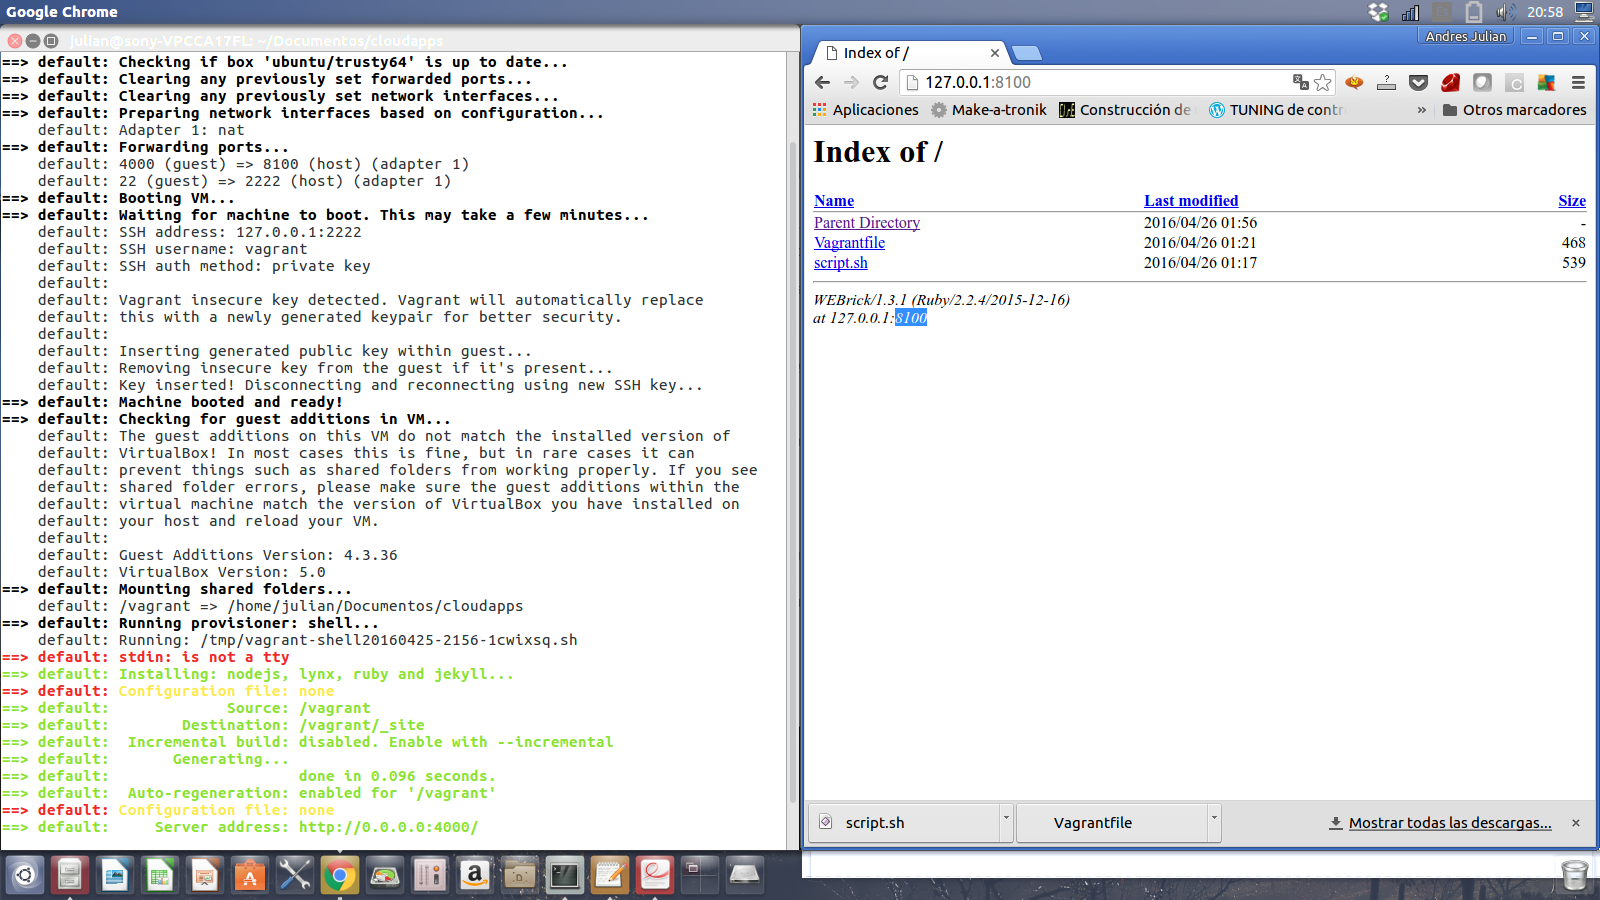
\includegraphics[scale=0.25]{despliegue}   
	\caption{  Acceso en un navegador (browser)} \label{fig:despliegue}
\end{figure}

\end{itemize}

\newpage % Se utiliza para escribir en una nueva pagina (estilo)
		
\section{Taller 4 - IaaS - Fundamentos de Vagrant - Parte II}

El objetivo del cuarto taller, continua el despliegue desarrollado en el taller No 3 sobre entornos de desarrollo sencillos mediante la tecnología Vagrant utilizando como proveedor de infraestructura la tecnología VirtualBox.
		
\begin{itemize}		

\item Abrir una consola de comandos. 
\item Validar la correcta instalación del software Vagrant ejecutando el comando "vagrant –h"
\begin{figure}[ht] 
	\centering
		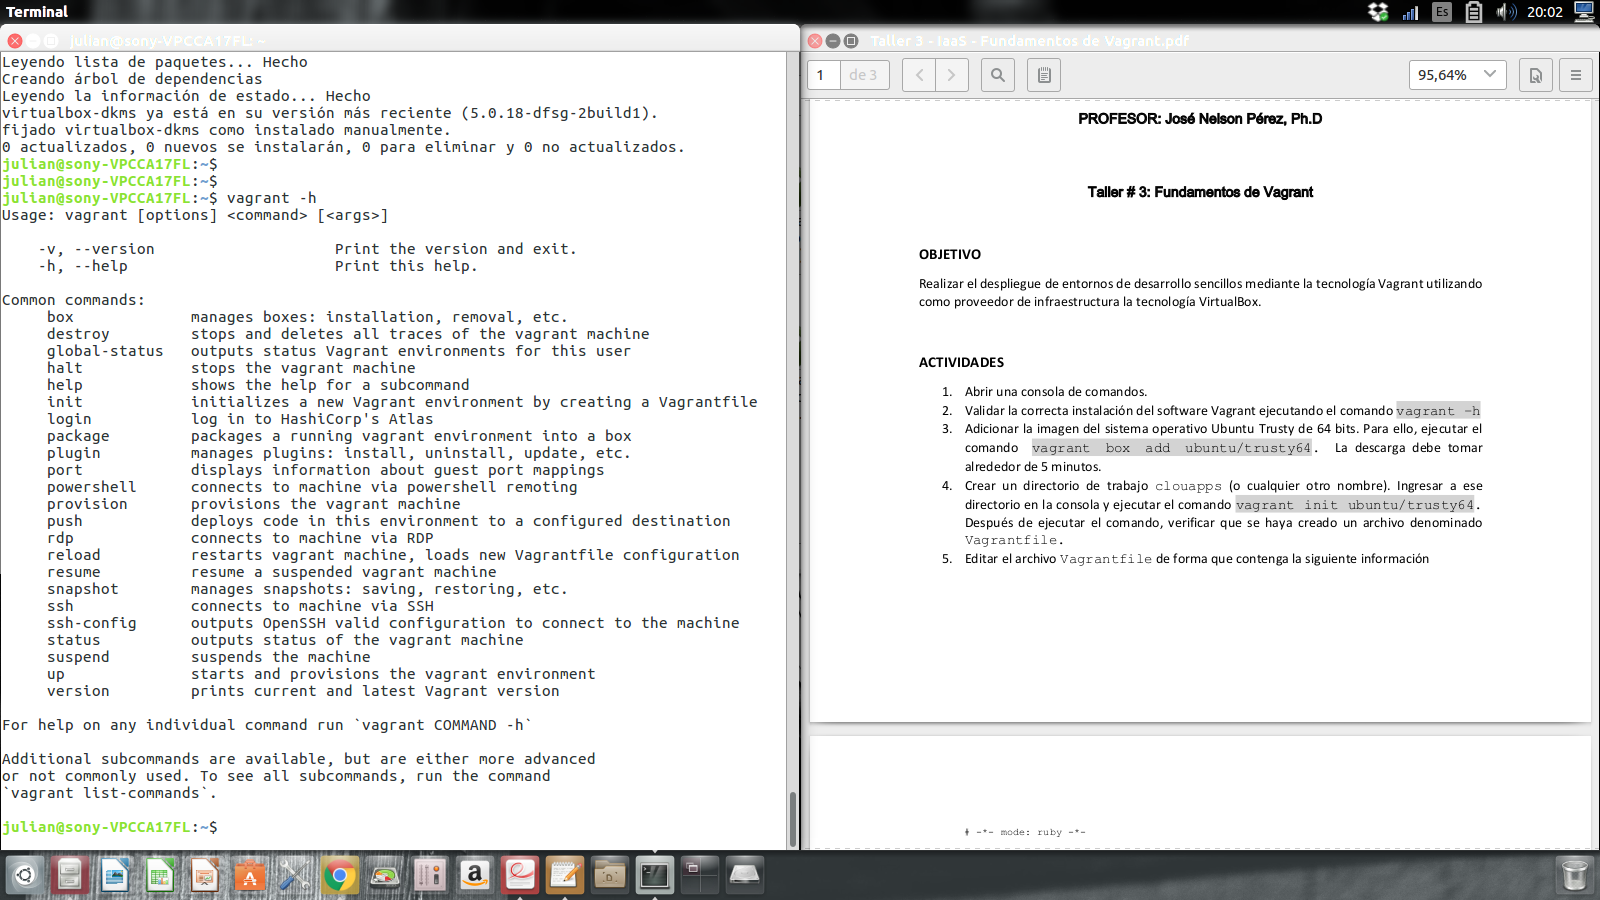
\includegraphics[scale=0.25]{vagrantverification}   
	\caption{Validación de la correcta instalación del software Vagrant} \label{fig:vagrantverification}
\end{figure}

\item Adicionar la imagen del sistema operativo Ubuntu Trusty de 64 bits. Para ello, ejecutar el comando "vagrant box add ubuntu/trusty64". La descarga debe tomar alrededor de 5 minutos.
\begin{figure}[ht] 
	\centering
		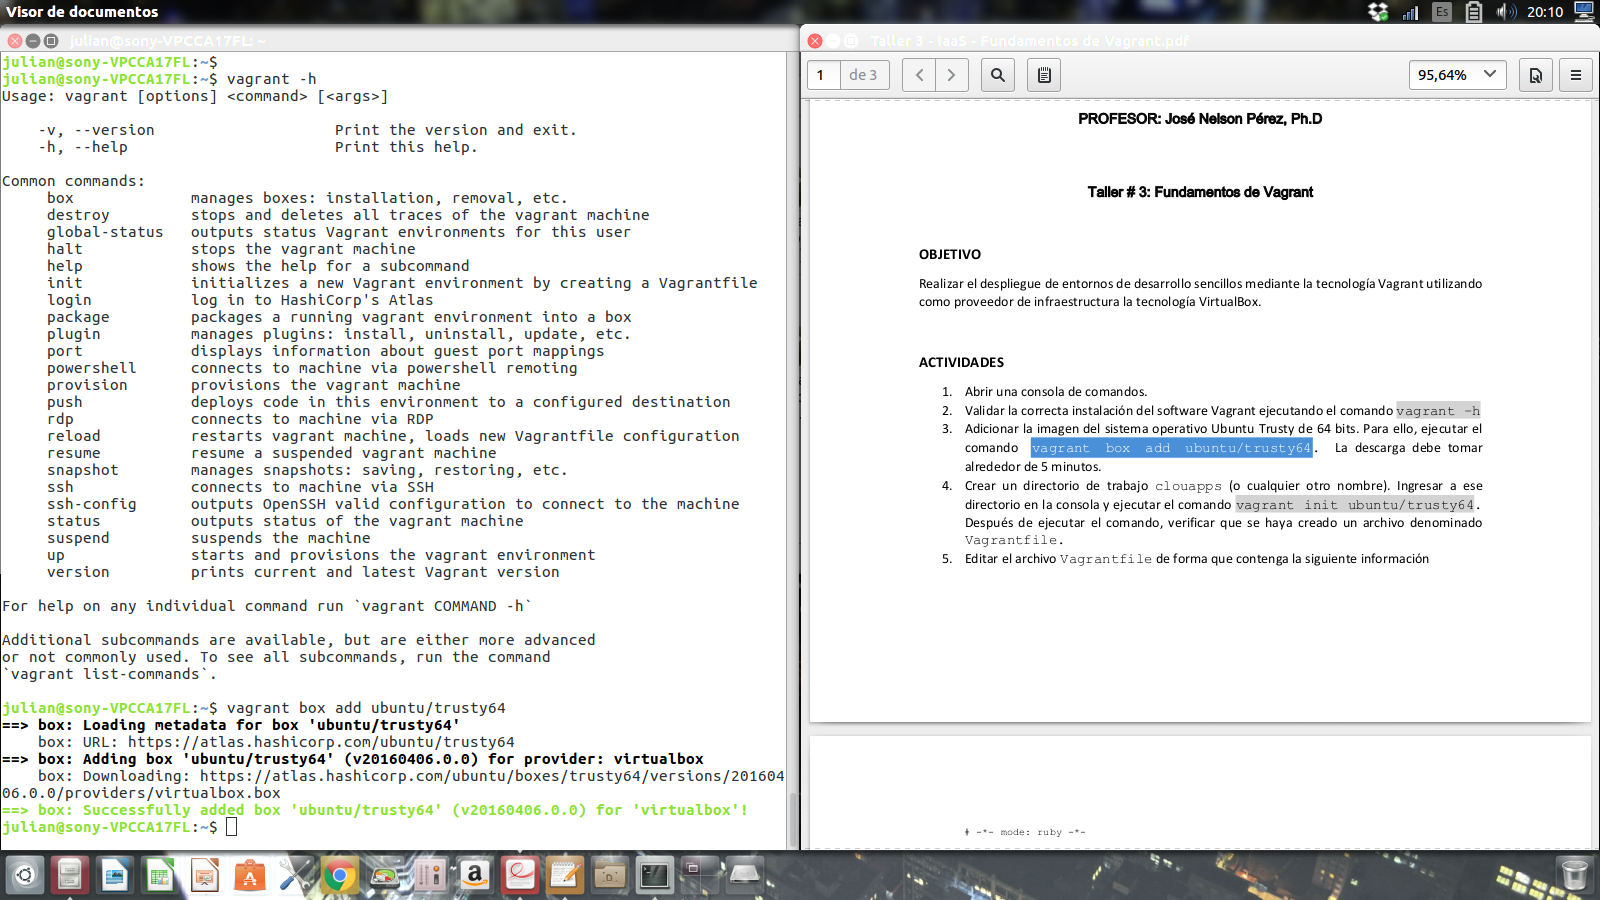
\includegraphics[scale=0.25]{bajadoubuntu}   
	\caption{Imagen del sistema operativo Ubuntu} \label{fig:bajadoubuntu}
\end{figure}

\item Crear un directorio de trabajo clouapps (o cualquier otro nombre). Ingresar a ese directorio en la consola y ejecutar el comando "vagrant init ubuntu/trusty64". Después de ejecutar el comando, verificar que se haya creado un archivo denominado "Vagrantfile".
\begin{figure}[ht] 
	\centering
		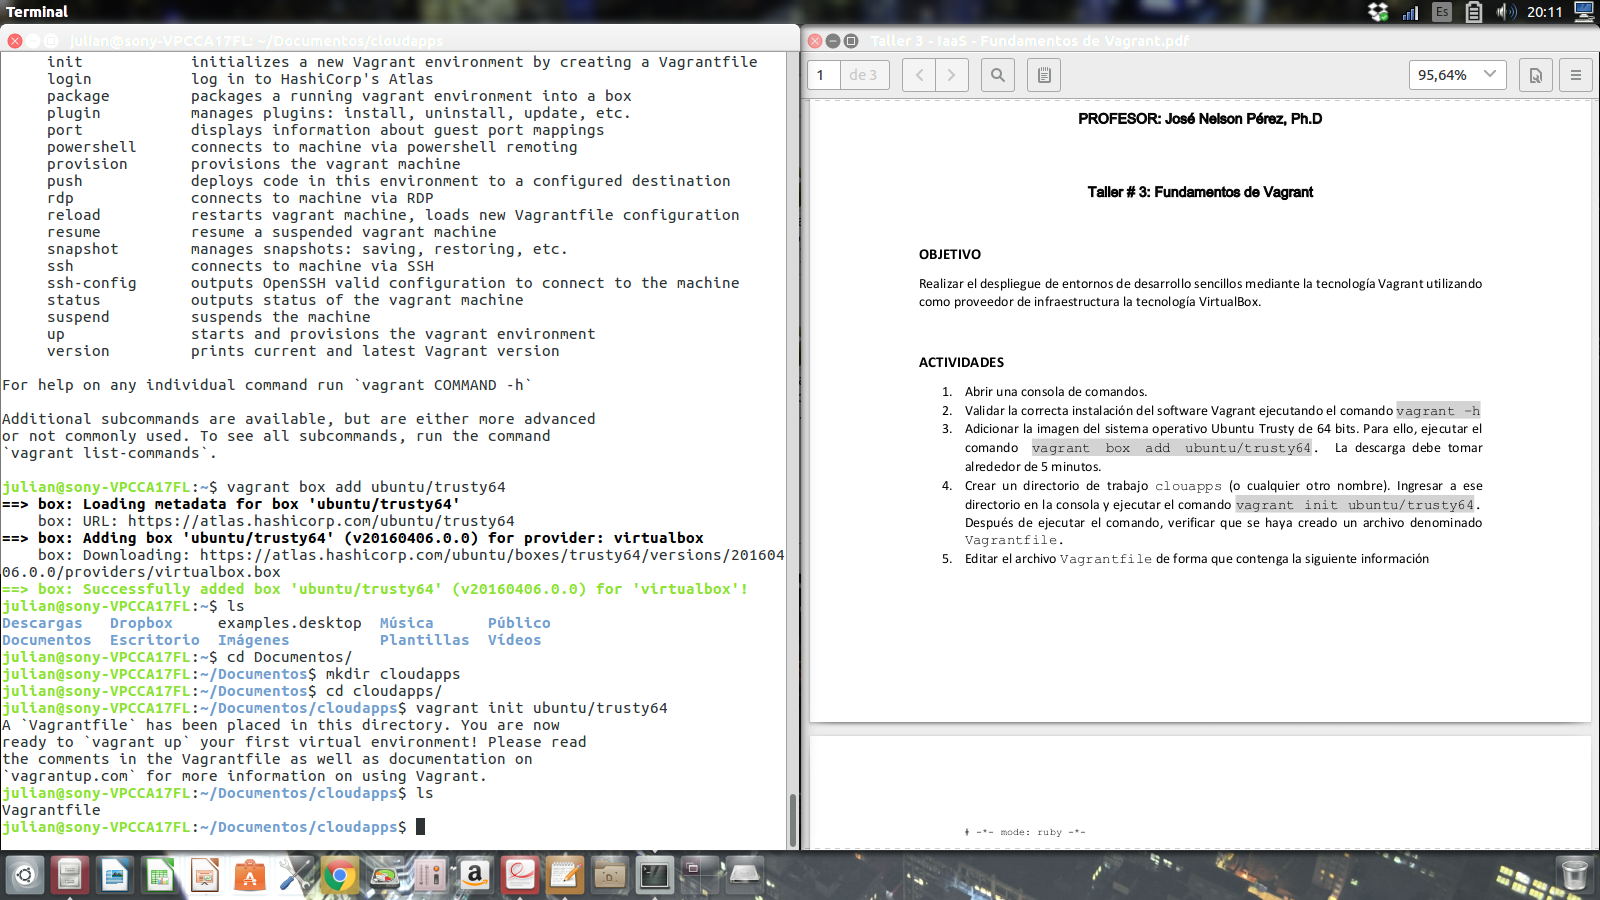
\includegraphics[scale=0.25]{vagrantfile}   
	\caption{ Creación del archivo denominado "Vagrantfile"} \label{fig:vagrantfile}
\end{figure}

\item Editar el archivo "Vagrantfile" de forma que contenga la siguiente información
	\begin{small}
	\begin{lstlisting}[frame=single,style=base]	
# -*- mode: ruby -*-
# vi: set ft=ruby :
# All Vagrant configuration is done below. The "2" in Vagrant.configure
# configures the configuration version (we support older styles for
# backwards compatibility). Please don't change it unless you know what
# you're doing.
Vagrant.configure(2) do |config|
config.vm.box = "ubuntu/trusty64"
config.vm.network :forwarded_port, guest: 4000, host: 8100, host_ip: "127.0.0.1"
config.vm.provision "shell", path: "script.sh"
end
	\end{lstlisting}
	\end{small}

\item Crear un archivo “default.pp” en un directorio manifests que se encuentra en el mismo lugar del archivo "Vagrantfile".
\item Escribir el siguiente contenido en el archivo “default.pp”.
	
	\begin{small}
	\begin{lstlisting}[frame=single,style=base]	
exec { 'apt-get update':
command => '/usr/bin/apt-get update -y'
}
package { 'nodejs':
require => Exec['apt-get update']
}
package { 'lynx-cur':
require => Exec['apt-get update']
}
package { 'ruby1.9.1-dev':
require => Exec['apt-get update']
}
	\end{lstlisting}
	\end{small}

\item Ejecutar el comando "vagrant up --provision".
\begin{figure}[ht] 
	\centering
		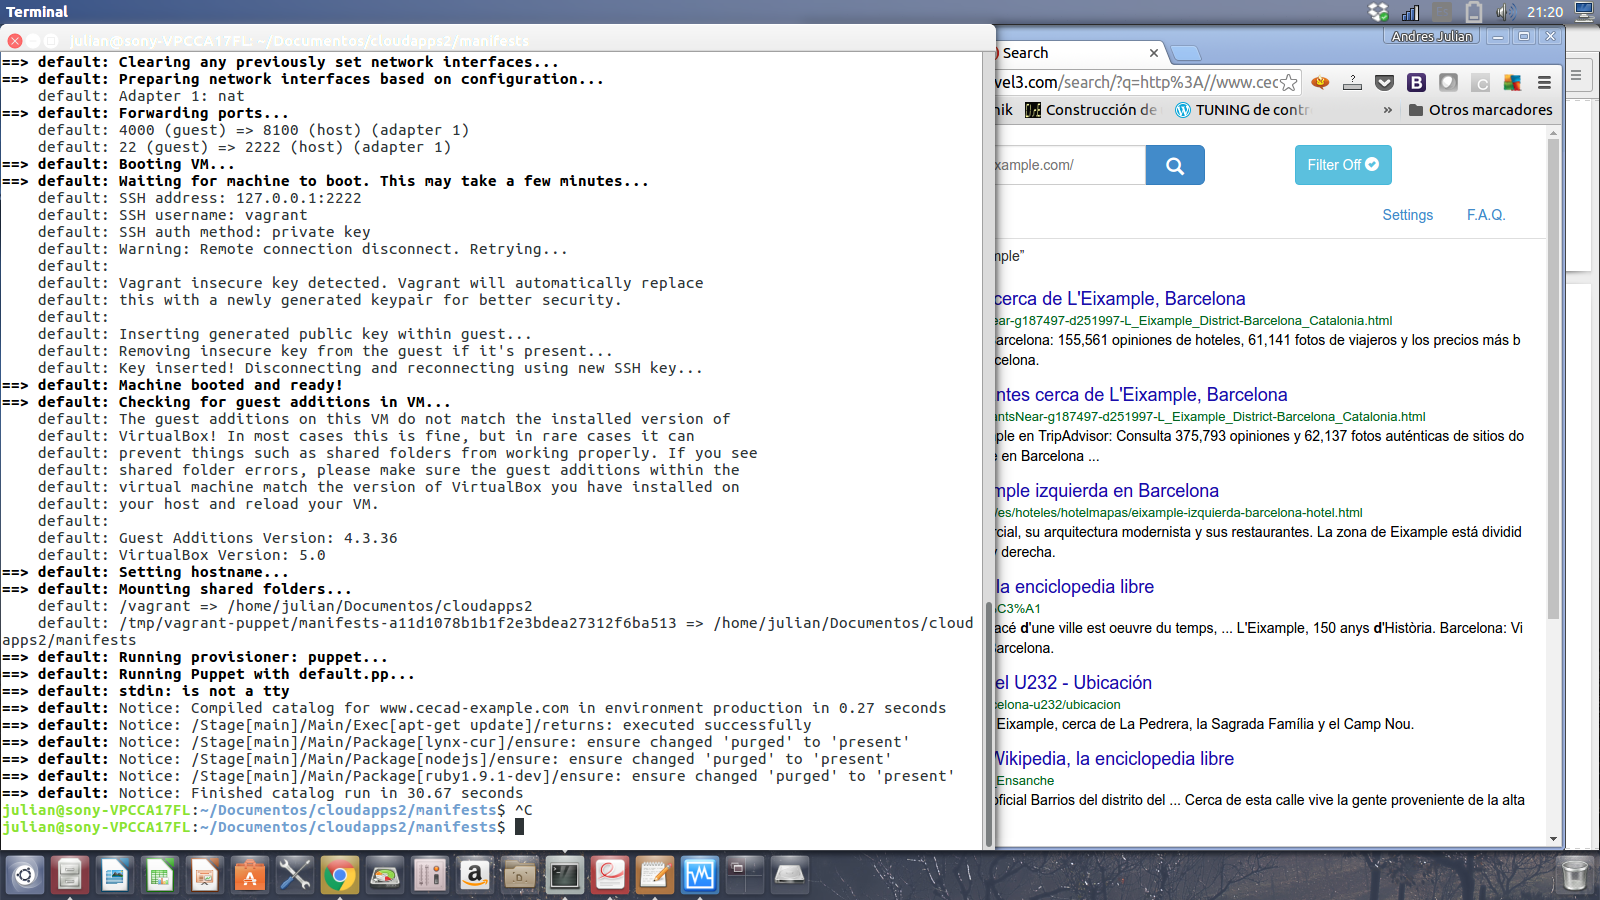
\includegraphics[scale=0.25]{deslplieguetaller4}   
	\caption{Resultado obtenido en el despliegue} \label{fig:deslplieguetaller4}
\end{figure}

\end{itemize}

\newpage % Se utiliza para escribir en una nueva pagina (estilo)

\section{Taller 6 - IaaS - Fundamentos de Docker}	
	
El objetivo del sexto taller, es realizar el despliegue de aplicaciones sencillas mediante la tecnología Docker sobre el sistema operativo Linux Ubuntu Server.

\begin{itemize}
		
\item Verificar la correcta instalación del servicio Docker ejecutando el comando
\begin{small}
\begin{lstlisting}[frame=single,style=base]	
	&sudo service docker status&
\end{lstlisting}
\end{small}
\begin{figure}[ht] 
	\centering
		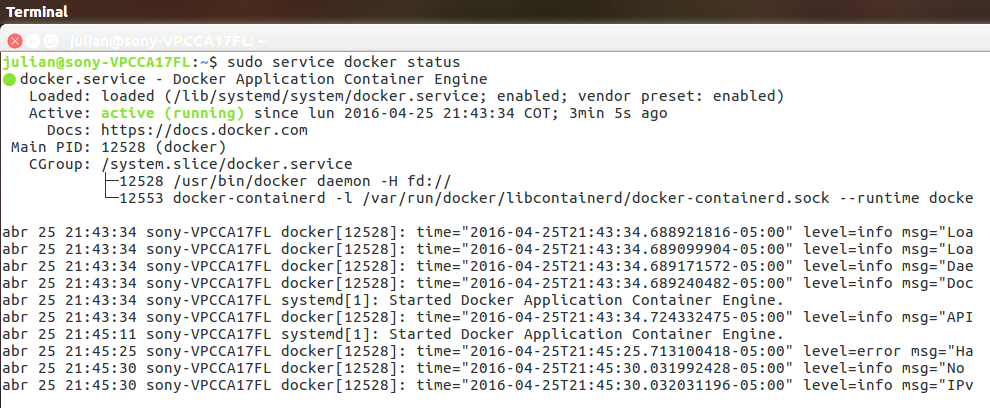
\includegraphics[scale=0.53]{dockerstatus}   
	\caption{Instalación del Docker} \label{fig:dockerstatus}
\end{figure}

\item Descargar la imagen oficial de Docker para el software Apache Solr (Motor de búsqueda de código abierto)
\begin{small}
\begin{lstlisting}[frame=single,style=base]	
	&sudo docker pull solr&
\end{lstlisting}
\end{small}
\begin{figure}[ht] 
	\centering
		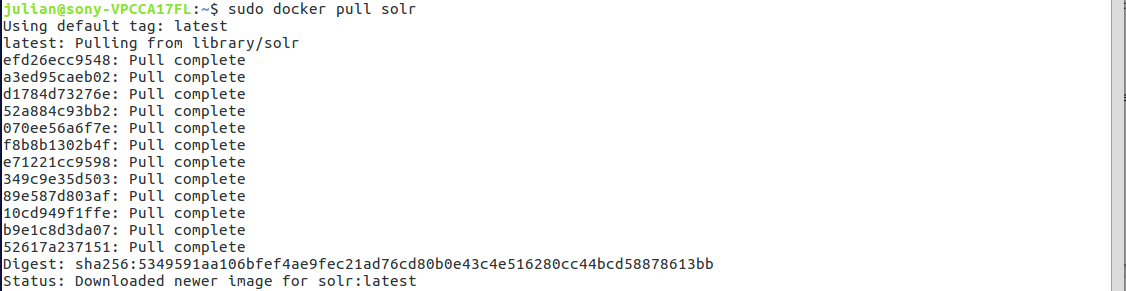
\includegraphics[scale=0.46]{dockerpullsolr}   
	\caption{Instalación de imagen oficial de Docker} \label{fig:dockerpullsolr}
\end{figure}

\item Listar las imágenes de Docker disponibles. Debe aparecer la imagen de solr descargada.
\begin{small}
\begin{lstlisting}[frame=single,style=base]	
	&sudo docker images&
\end{lstlisting}
\end{small}
\begin{figure}[ht] 
	\centering
		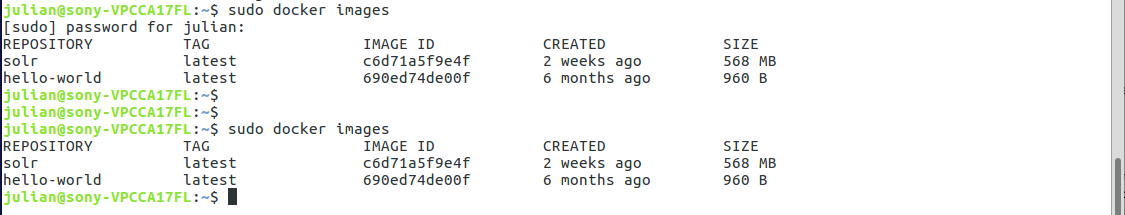
\includegraphics[scale=0.46]{dockerimages}   
	\caption{Listar las imágenes de Docker} \label{fig:dockerimages}
\end{figure}

\item Iniciar el servidor de Apache Solr ejecutando un contenedor de Docker.
\begin{small}
\begin{lstlisting}[frame=single,style=base]	
	&sudo docker run p 8983:8983 d name mysolr solr&
\end{lstlisting}
\end{small}
\begin{figure}[ht] 
	\centering
		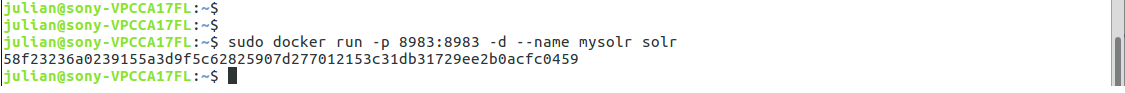
\includegraphics[scale=0.46]{dockerrun}   
	\caption{Iniciar el servidor de Apache Solr} \label{fig:dockerrun}
\end{figure}

\item Verificar que el contenedor se esté ejcutando. Para ello, ejecutar el comando
\begin{small}
\begin{lstlisting}[frame=single,style=base]	
	&sudo docker ps&
\end{lstlisting}
\end{small}

\item En el anterior comando, se listan varias características del contenedor, incluido su identificador. Con este identificador, es posible acceder a los logs del contenedor, si es necesario verificar en detalle las acciones sobre el mismo.
\begin{small}
\begin{lstlisting}[frame=single,style=base]	
	&sudo docker logs f <id-contenedor>&
\end{lstlisting}
\end{small}
\begin{figure}[ht] 
	\centering
		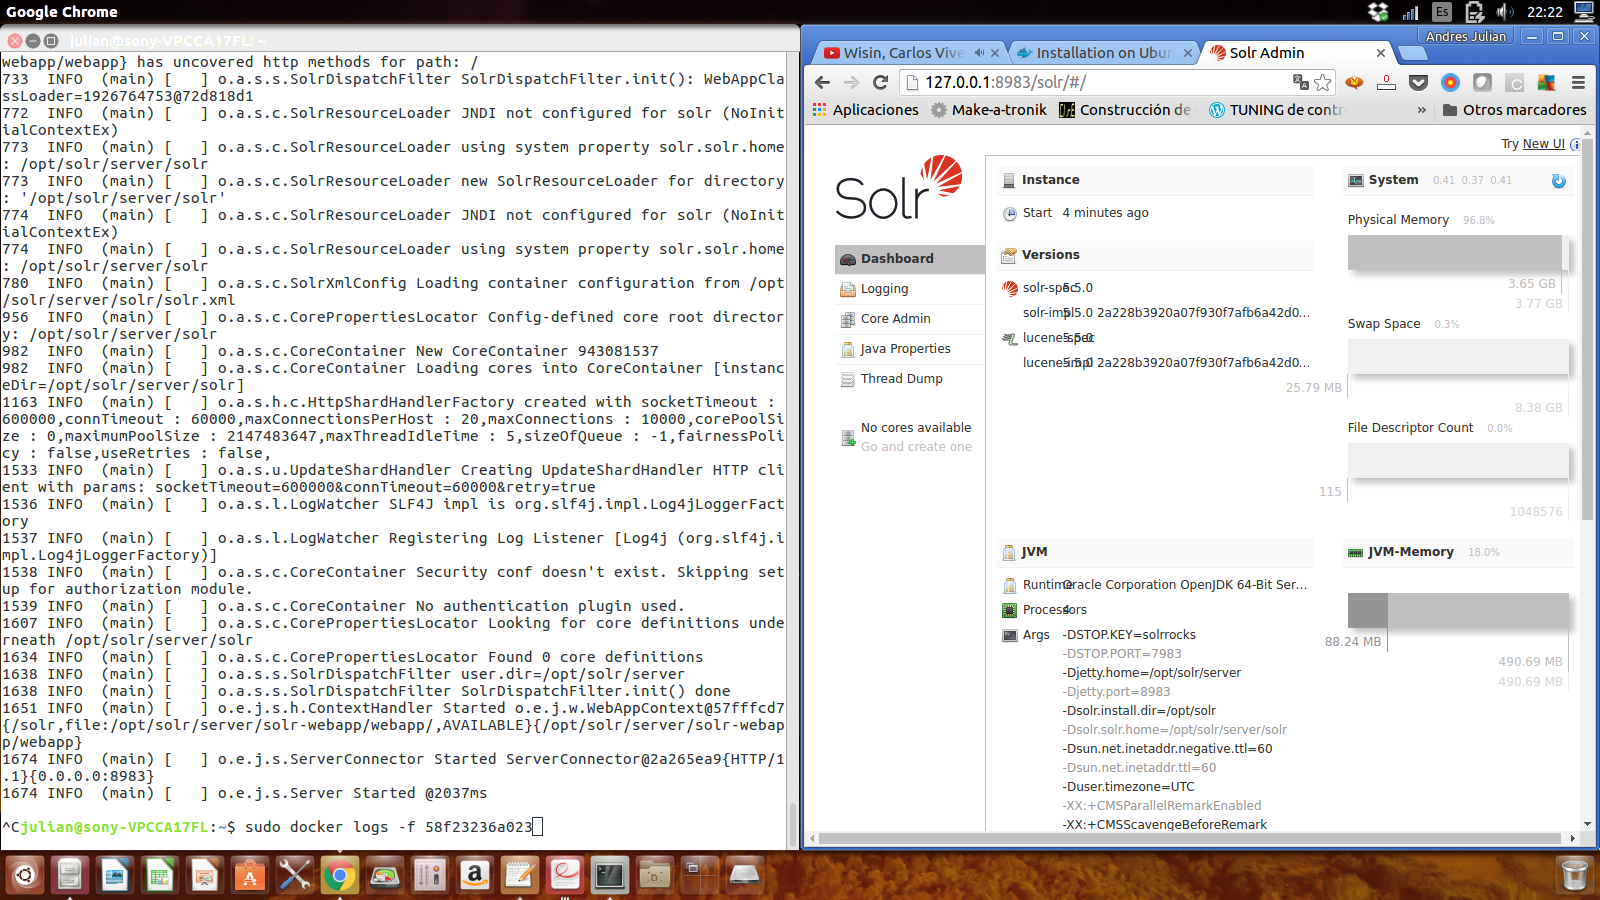
\includegraphics[scale=0.25]{dockerlogs}   
	\caption{Logs del contenedor} \label{fig:dockerlogs}
\end{figure}

\item Acceder a la consola de administración del servidor Apache Solr. Para ello, desde un navegador ingresar a la URL http://"direccion-huesped-docker":89983

\item En este momento, la aplicación ya está desplegada en el contenedor, disponible para utilización. Por ejemplo, se desea utilizar el servidor Solr recién desplegado para crear un índice núcleo. Lo primero es acceder a la consola del contenedor, ya que este se encuentra ejecutándose como un proceso en "background".
\begin{small}
\begin{lstlisting}[frame=single,style=base]	
	&sudo docker exec it user=solr mysolr bash&
\end{lstlisting}
\end{small}
\begin{figure}[ht] 
	\centering
		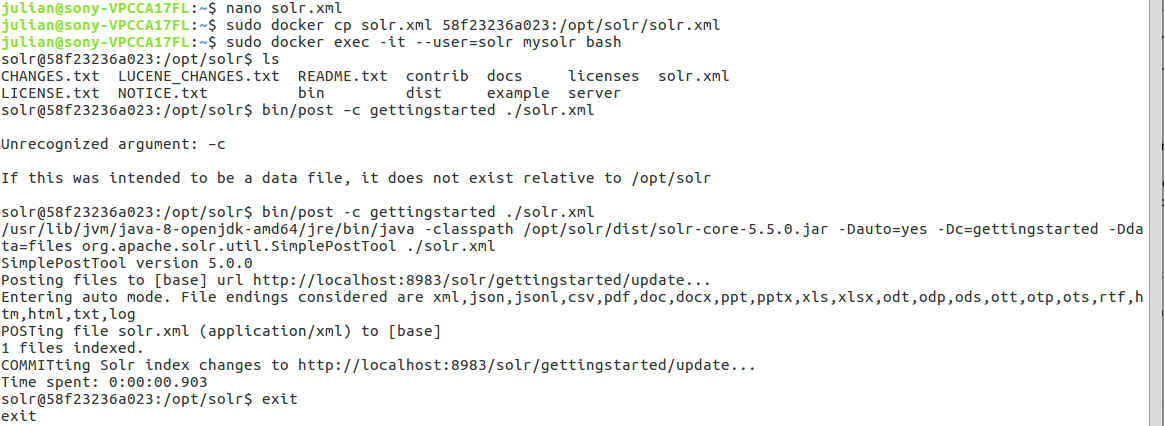
\includegraphics[scale=0.48]{dockerexec}   
	\caption{Acceso a la consola del contenedor} \label{fig:dockerexec}
\end{figure}

\item Ejecutar el comando
\begin{small}
\begin{lstlisting}[frame=single,style=base]	
	&bin/solr create_core c gettingstarted&
\end{lstlisting}
\end{small}
\begin{figure}[ht] 
	\centering
		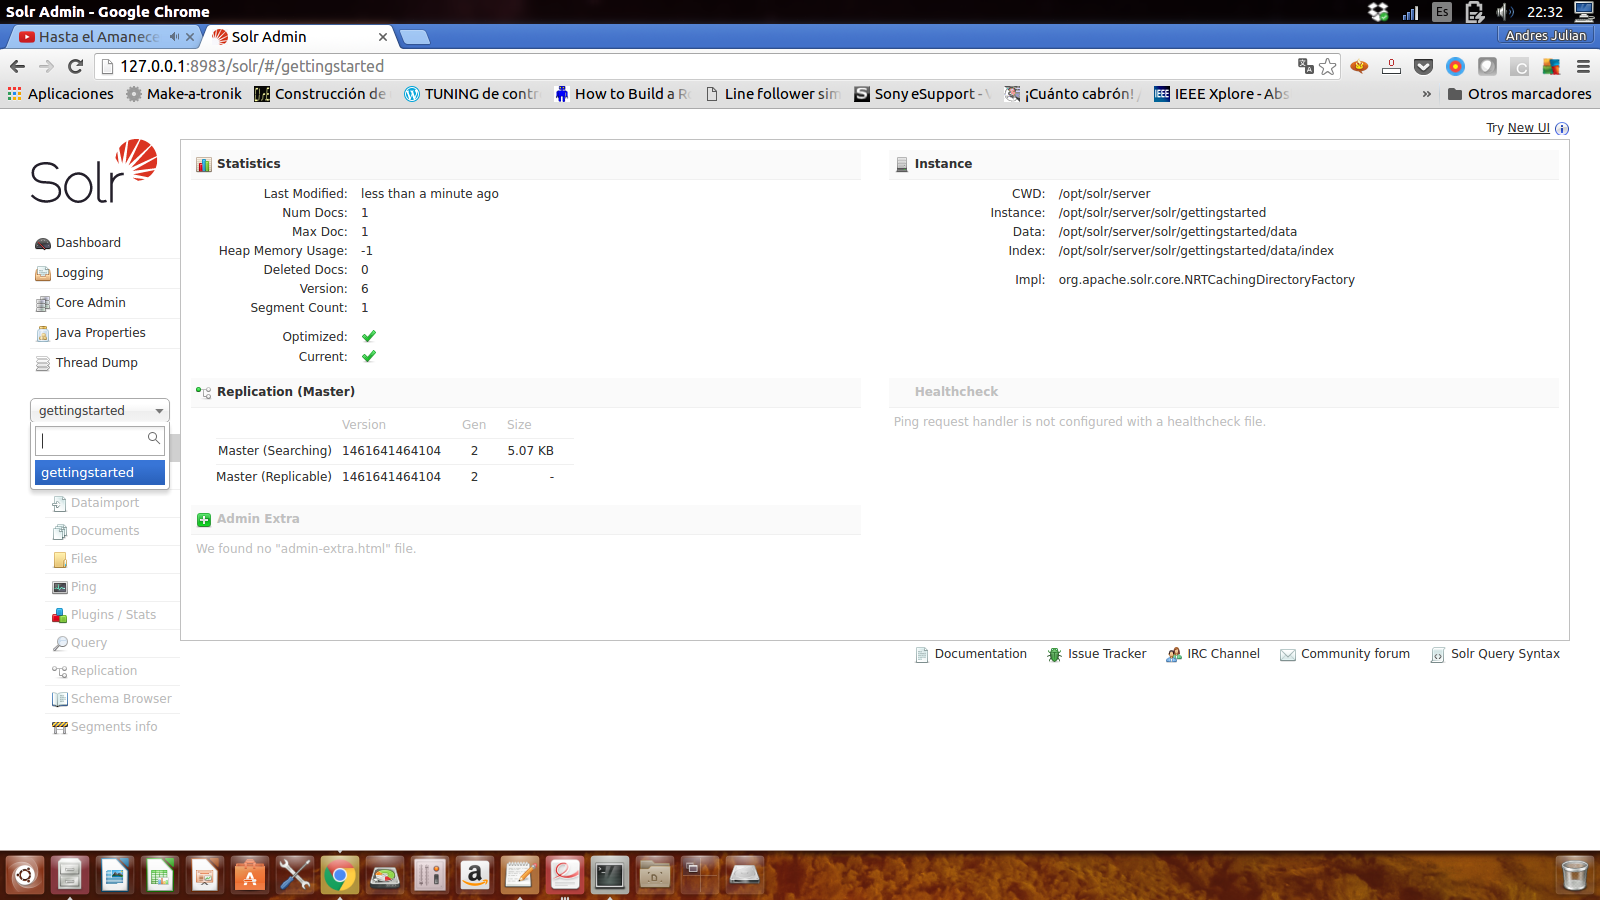
\includegraphics[scale=0.26]{getingstartedsolr}   
	\caption{Creación de un índice núcleo} \label{fig:getingstartedsolr}
\end{figure}

\item Una de las funcionalidades más interesantes de Docker es poder copiar directamente un archivo creado en la máquina huésped a cualquier directorio dentro del contenedor. Para ello, crear en la máquina huésped (no en el contenedor) un archivo solr.xml con el siguiente contenido a manera de ejemplo:
\begin{small}
\begin{lstlisting}[frame=single,style=base]	
<add>
	<doc>
		<field name="id">SOLR1000</field>
		<field name="name">Solr, the Enterprise Search Server</field>
		<field name="manu">Apache Software Foundation</field>
		<field name="cat">software</field>
		<field name="cat">search</field>
		<field name="features">Advanced Full-Text Search Capabilities using Lucene</field>
		<field name="features">Optimized for High Volume Web Traffic</field>
		<field name="features">Standards Based Open Interfaces - XML and HTTP</field>
		<field name="features">Comprehensive HTML Administration Interfaces</field>
		<field name="features">Scalability - Efficient Replication to other Solr Search Servers</field>
		<field name="features">Flexible and Adaptable with XML configuration and Schema</field>
		<field name="features">Good unicode support: h#xE9;llo (hello with an accent over the e)</field>
		<field name="price">0</field>
		<field name="popularity">10</field>
		<field name="inStock">true</field>
		<field name="incubationdate_dt">2006-01-17T00:00:00.000Z</field>
	</doc>
</add>
\end{lstlisting}
\end{small}

Acto seguido, copiar el archivo al directorio /opt/solr en el contenedor. Reemplazar "id-contenedor" con el respectivo valor.

\begin{small}
\begin{lstlisting}[frame=single,style=base]	
	&sudo docker cp solr.xml <idcontenedor>:/opt/solr/solr.xml&
\end{lstlisting}
\end{small}

\item Ingresar nuevamente a la consola. Verificar la existencia del archivo solr.xml y ejecutar el comando
\begin{small}
\begin{lstlisting}[frame=single,style=base]	
	&bin/post c gettingstarted ./solr.xml&
\end{lstlisting}
\end{small}
\begin{figure}[ht] 
	\centering
		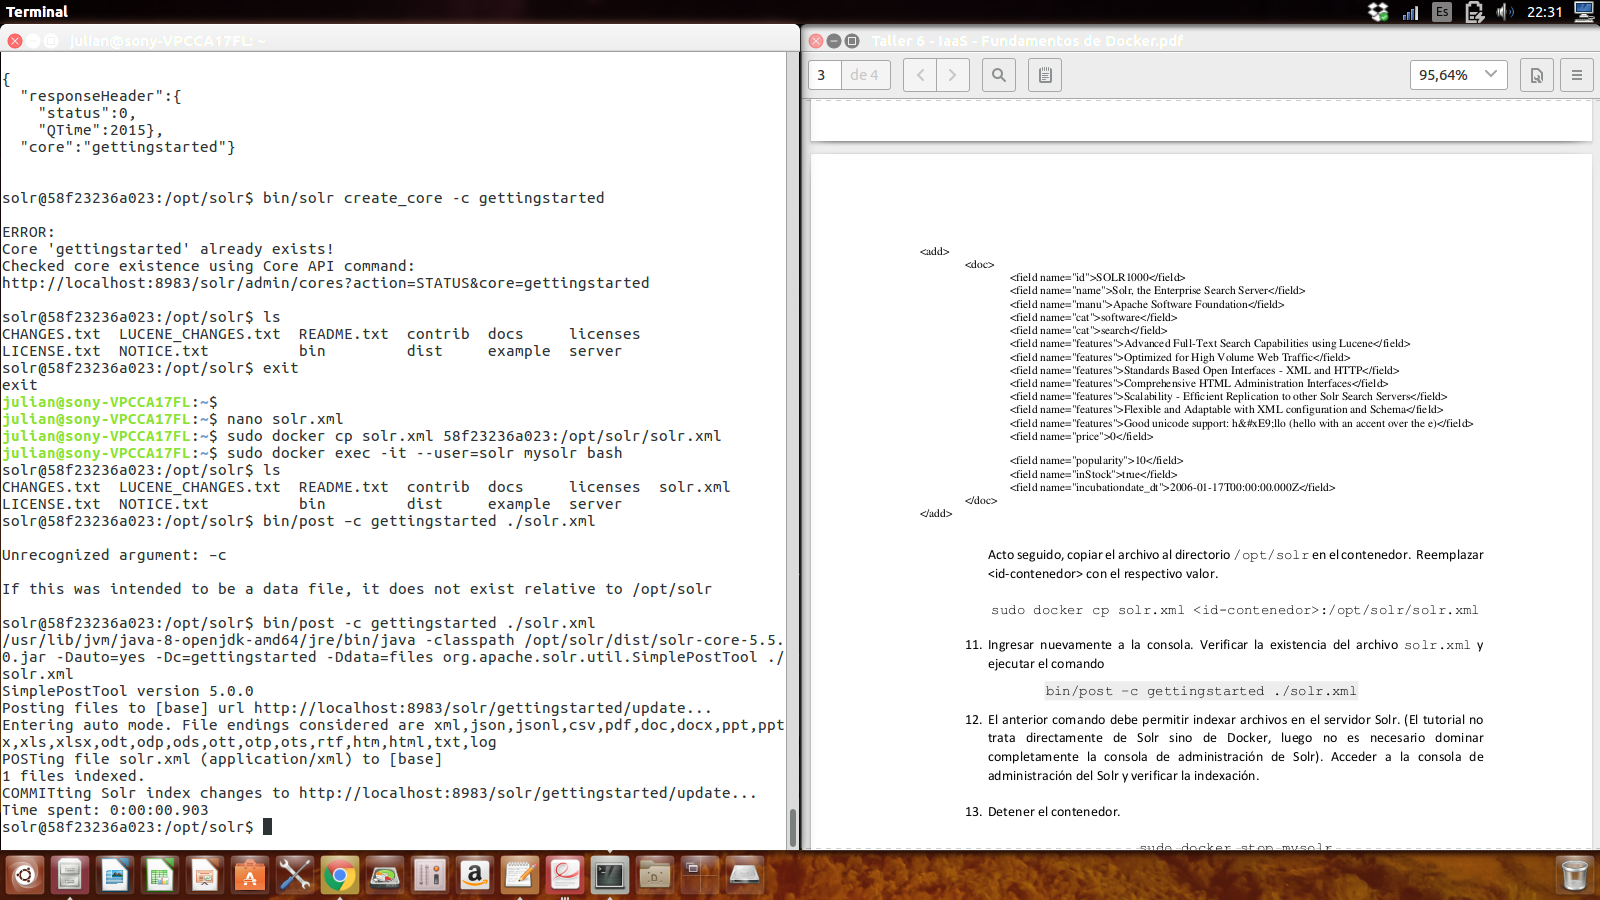
\includegraphics[scale=0.26]{solrxml}   
	\caption{Creación de un archivo solr.xml} \label{fig:solrxml}
\end{figure}

\item El anterior comando debe permitir indexar archivos en el servidor Solr. (El tutorial no trata directamente de Solr sino de Docker, luego no es necesario dominar completamente la consola de administración de Solr). Acceder a la consola de administración del Solr y verificar la indexación.

\item Detener el contenedor.
\begin{small}
\begin{lstlisting}[frame=single,style=base]	
	&sudo docker stop mysolr&
\end{lstlisting}
\end{small}

Verificar que el contenedor aparezca como “Exited” en su estado después de ejecutar el comando

\begin{small}
\begin{lstlisting}[frame=single,style=base]	
	&sudo docker ps a&
\end{lstlisting}
\end{small}
\begin{figure}[ht] 
	\centering
		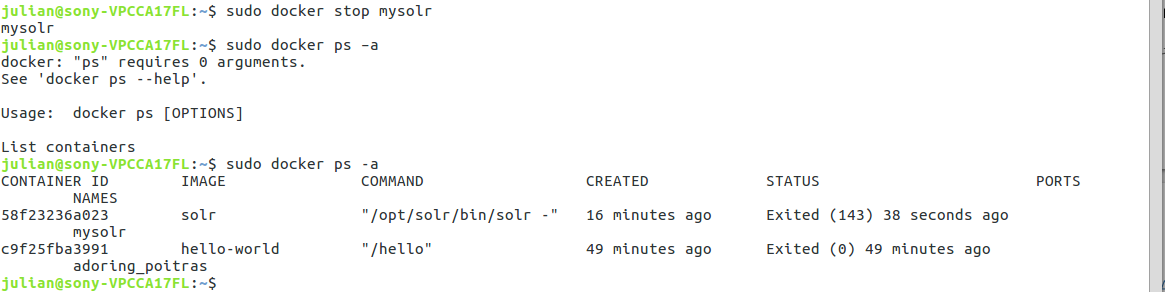
\includegraphics[scale=0.48]{apagandosolr}   
	\caption{Detener el contenedor} \label{fig:apagandosolr}
\end{figure}

\item Eliminar el contenedor.
\begin{small}
\begin{lstlisting}[frame=single,style=base]	
	&sudo docker rm mysolr&
\end{lstlisting}
\end{small}

\item En caso de requerirse, es posible eliminar la imagen utilizando el comando
\begin{small}
\begin{lstlisting}[frame=single,style=base]	
	&sudo docker rmi solr&
\end{lstlisting}
\end{small}

\end{itemize}

\newpage 

\section{Taller 7 - IaaS - Fundamentos de Docker - Parte II}

El objetivo del septimo taller, radica en darle continuidad al despliegue de aplicaciones sencillas utilizando la tecnología Docker sobre el sistema operativo Linux Ubuntu Server.

\begin{itemize}

\item Verificar la correcta instalación del servicio Docker ejecutando el comando
\begin{small}
\begin{lstlisting}[frame=single,style=base]	
	&sudo service docker status&
\end{lstlisting}
\end{small}
\begin{figure}[ht] 
	\centering
		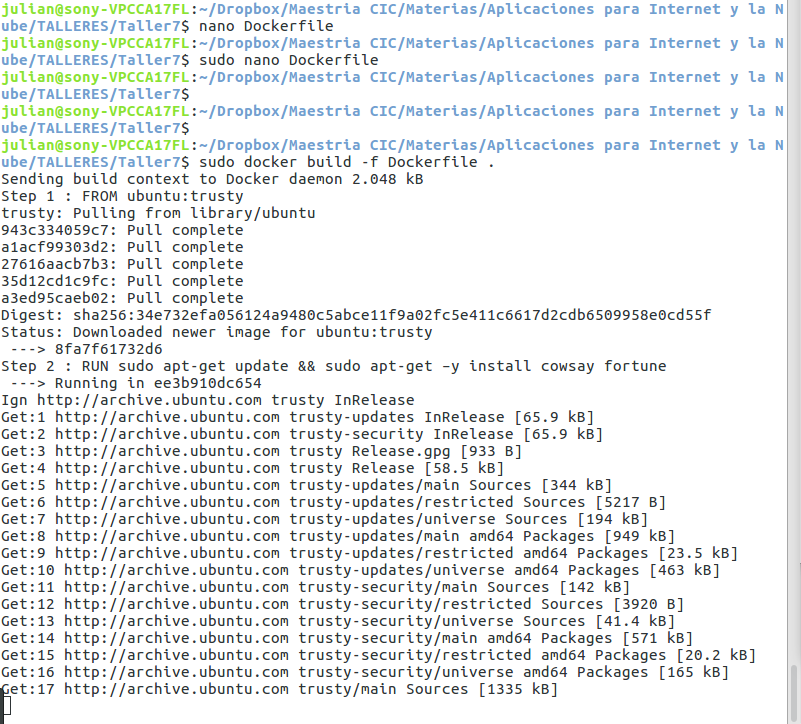
\includegraphics[scale=0.6]{docker}   
	\caption{Instalación del servicio Docker} \label{fig:docker}
\end{figure}

\item En este taller se va a utilizar un archivo denominado Dockerfile (similar al Vagrafile) que establece el conjunto de pasos para desplegar una imagen Docker. Crear un directorio, entrar a ese directorio y crear un archivo llamado “Dockerfile”.

\item Ingresar el siguiente contenido en el archivo:
\begin{small}
\begin{lstlisting}[frame=single,style=base]	
	&FROM& Ubuntu:trusty
	&RUN& sudo apt-get update && sudo apt-get y install cowsay fortune
\end{lstlisting}
\end{small}

\item Construir una nueva imagen a partir del Dockerfile.
\begin{small}
\begin{lstlisting}[frame=single,style=base]	
	&sudo docker build t test/dockerfile-example&
\end{lstlisting}
\end{small}
\begin{figure}[ht] 
	\centering
		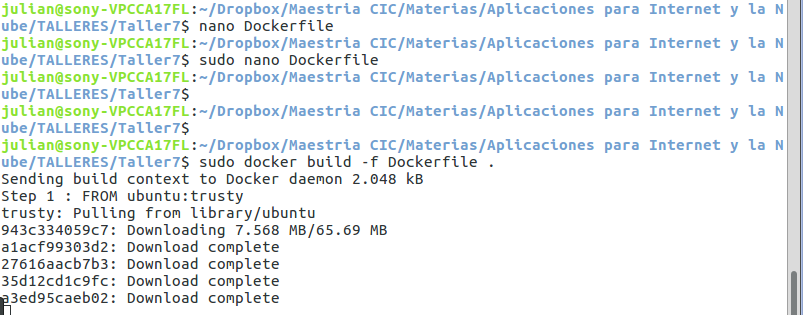
\includegraphics[scale=0.7]{creandoimagen}   
	\caption{Construcción de una nueva imagen a partir del archivo "Dockerfile"} \label{fig:creandoimagen}
\end{figure}

\item  Ejecutar un nuevo contenedor a partir de la imagen creada.
\begin{small}
\begin{lstlisting}[frame=single,style=base]	
	&sudo docker run test/dockerfile-example /usr/games/cowsay& 'Hola a todos'
\end{lstlisting}
\end{small}
\begin{figure}[ht] 
	\centering
		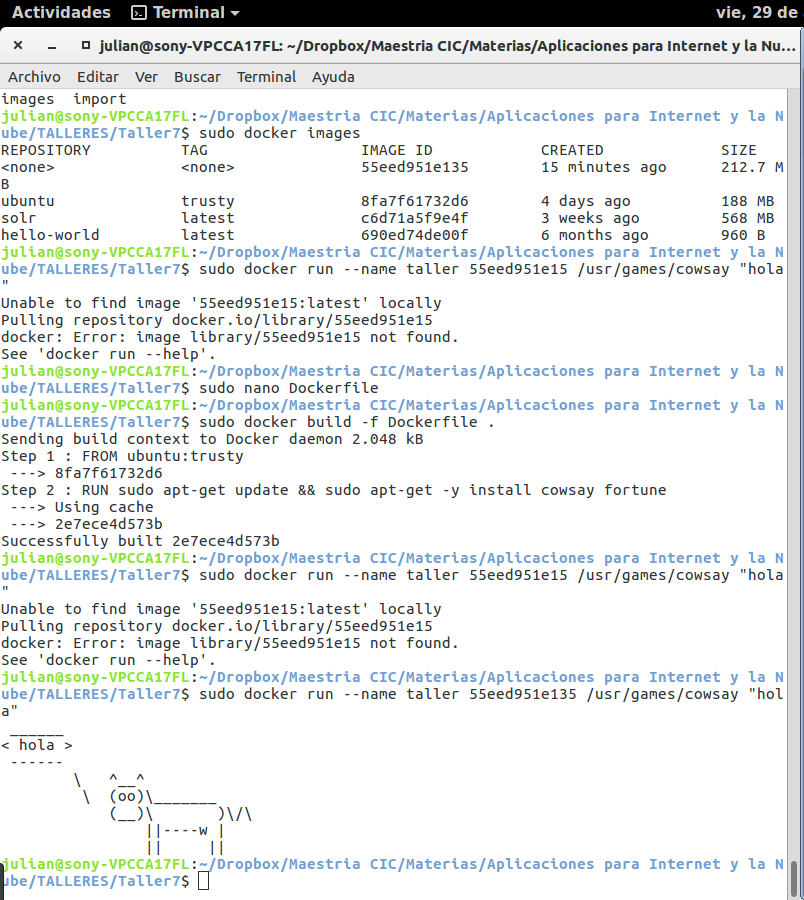
\includegraphics[scale=0.6]{dockerfile}   
	\caption{Creación de la imagen a partir del archivo “Dockerfile”} \label{fig:dockerfile}
\end{figure}

\end{itemize}

\end{document}
